% --------------------------------------------------------------
% This is all preamble stuff that you don't have to worry about.
% Head down to where it says "Start here"
% --------------------------------------------------------------
 
\documentclass[12pt]{article}
 
\usepackage[margin=1in]{geometry} 
\usepackage{amsmath,amsthm,amssymb, graphicx, verbatim}
 \usepackage{algorithm}
\usepackage{algorithmic}
\usepackage{hyperref}
\newcommand{\N}{\mathbb{N}}
\newcommand{\Z}{\mathbb{Z}}
 
\newenvironment{theorem}[2][Theorem]{\begin{trivlist}
\item[\hskip \labelsep {\bfseries #1}\hskip \labelsep {\bfseries #2.}]}{\end{trivlist}}
\newenvironment{lemma}[2][Lemma]{\begin{trivlist}
\item[\hskip \labelsep {\bfseries #1}\hskip \labelsep {\bfseries #2.}]}{\end{trivlist}}
\newenvironment{exercise}[2][Exercise]{\begin{trivlist}
\item[\hskip \labelsep {\bfseries #1}\hskip \labelsep {\bfseries #2.}]}{\end{trivlist}}
\newenvironment{problem}[2][Problem]{\begin{trivlist}
\item[\hskip \labelsep {\bfseries #1}\hskip \labelsep {\bfseries #2.}]}{\end{trivlist}}
\newenvironment{question}[2][Question]{\begin{trivlist}
\item[\hskip \labelsep {\bfseries #1}\hskip \labelsep {\bfseries #2.}]}{\end{trivlist}}
\newenvironment{corollary}[2][Corollary]{\begin{trivlist}
\item[\hskip \labelsep {\bfseries #1}\hskip \labelsep {\bfseries #2.}]}{\end{trivlist}}

\newenvironment{solution}{\begin{proof}[Solution]}{\end{proof}}

\def\code#1{\texttt{#1}}

\begin{document}
\nocite{*} 
% --------------------------------------------------------------
%                         Start here
% --------------------------------------------------------------
 

\title{GPU Sparse Matrix Multiplication}
\author{Xingyou Song, \footnote{xsong@berkeley.edu} Nitin Manivasagan, \footnote{nitinmani@berkeley.edu} Manar Safi \footnote{safi.manar@berkeley.edu}}
\date{May 8, 2018} 
\maketitle

\section{Introduction}
Our code can be found on: \url{https://github.com/Srizzle/GPU-Sparse-Matrix-Multiply-CS-267}.

GPU-assisted sparse matrix operations have been well-known for a long time. In this report, we discuss the approaches of many of the well-known algorithms and perform experiments to benchmark and compare their performances on both random matrix-matrix multiplication. 

To avoid confusion, are separate naming conventions for each case when dealing with matrix-multiplication. These are: 
\begin{itemize}
\item SpMV - (Sparse Matrix) $\times$ (Dense Vector) - Multiplications of form $M \cdot b$, where $M$ is a sparse matrix, and $b$ is a 1-d vector with any set of non-zero entries.
\item SpMM - (Sparse Matrix) $\times$ (Multiple Dense Vectors) - Multiplications of form $M \cdot N$, where $M$ is a sparse matrix, and $N$ is a matrix built by multiple dense vectors. 
\item SpGEMM (Sparse Matrix) $\times$ (Sparse Matrix) - Multiplications of form $M \cdot N$, where $M,N$ are both sparse matrices. 
\end{itemize}

Note that the libraries of interest, where each library may support some (or all) of these operations are:

\begin{itemize}
\item CUSP - Open Source wrapper library for open-source library Thrust: \url{https://github.com/cusplibrary/cusplibrary/tree/release/v0.6.0-rc} \footnote{The official release (4.0 and 5.0's do not work with our code) }
\item CuSPARSE - Production-level library: \url{https://developer.nvidia.com/cusparse} \footnote{Production libraries do not present the source code.}
\item CuBLAS - Production-level library: \url{https://developer.nvidia.com/cublas}
\end{itemize}

In the interest of time (as well as the fact that many open-source libraries are \textit{extremely} error-prone and unstable), we also considered the following libraries, but did not fully implement them due to heavy installation errors: \footnote{A large portion of our time was used in setting up different environments, because almost all open-source libraries are poorly documented, or have bugs.}
\begin{itemize}
\item bhSPARSE - Recent Modifications to original libraries: \url{https://github.com/bhSPARSE/bhSPARSE}
\item OpenAI Blocksparse - Open Source library for special "block-sparse" matrices: \url{https://github.com/openai/blocksparse} \footnote{We attempted to install all variants and versions on PSU XSEDE, Amazon AWS with Nvidia Tesla K80 (p2x.large instance), Amazon AWS with Nvidia Tesla P100 (p3x.large instance), Google Cloud Computing API with Nvidia Tesla P100, with no success on any of them}
\end{itemize}

To assist in readability in code, we used some wrapper libraries:
\begin{itemize}
\item CuBLAS - Cupy: \url{https://github.com/cupy/cupy}
\item CuSPARSE - PyCulib: \url{https://github.com/numba/pyculib}
\end{itemize}

The wrapper libraries that we attempted to use, but obsolete or failed are:
\begin{itemize}
\item CuSPARSE wrapper - Julia: \url{https://github.com/JuliaGPU/CUSPARSE.jl}
\item CuSPARSE wrapper - SkCUDA: \url{https://github.com/lebedov/scikit-cuda/tree/master/skcuda}
\end{itemize}

\section{Algorithmic Methods}
In this section we explain the common methods for sparse matrix multiplication, and link which methods to the correct libraries.

\subsection{SpMV}
From \cite{spmv_cuda}, there is an emphasis on the format representation of sparsity, which in turn is used to consider the appropriate GPU method. The goal is to compute $M \cdot b$. 3 methods are shown: 

\begin{itemize}
\item Diagonal format (structure specific) - For matrices $M$ whose elements are dominant on diagonals (close to the main diagonal), the matrix can represented by forming a data matrix (with zero-elements replaced as a "*" character), and an offset vector. The elements on the k-th column of the data matrix $D$ are matched with the k-th element of the offset vector, which specifies the diagonal on $M$. The elements on the data matrix are also row-aligned (i.e. elements of the same row in $M$ will also be in the same row in $D$). 

\begin{figure}[h]
  \caption{Diagonal format example}
  \centering 
  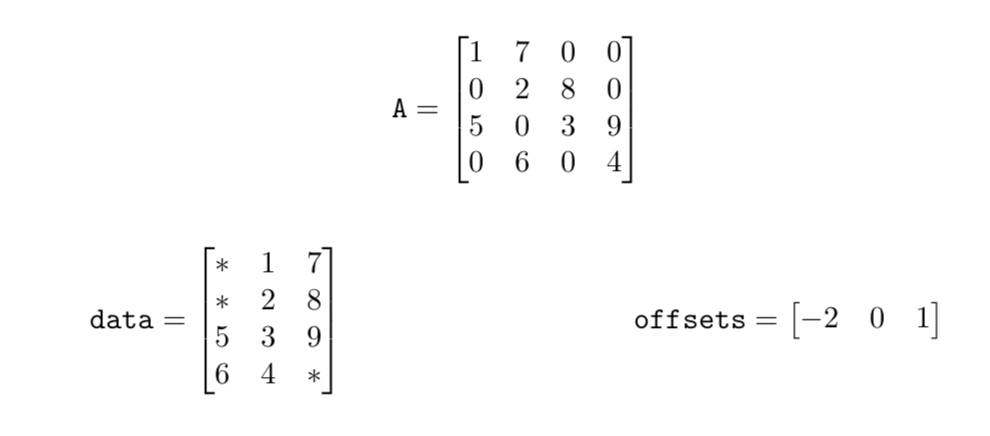
\includegraphics[width = 0.65\textwidth]{diagonal.png}
\end{figure}



For GPU computation, each thread $t$ will be responsible for computing the $t$-th element on the output (i.e. dot product between row $t$ in $M$ with the input vector). Because of the row alignment, each thread will contiguously access data along the row, incrementing the final output with $+= M[t][i]*B[i] $ for all $i$. 
\item ELLPACK format - This format is a general format, under the assumption that each row has a maximum of $Z$ non-zero elements in $M$. Intuitively, this then compacts $M$ into a data matrix, where each row $r$ of the data matrix is the list of non-zero elements of the row $r$ in $M$. The $r$-th row in the index matrix lists the column-coordinates of the elements in data at row $r$ with the elements in $M$. 


\begin{figure}[h]
  \caption{ELLPACK}
  \centering 
  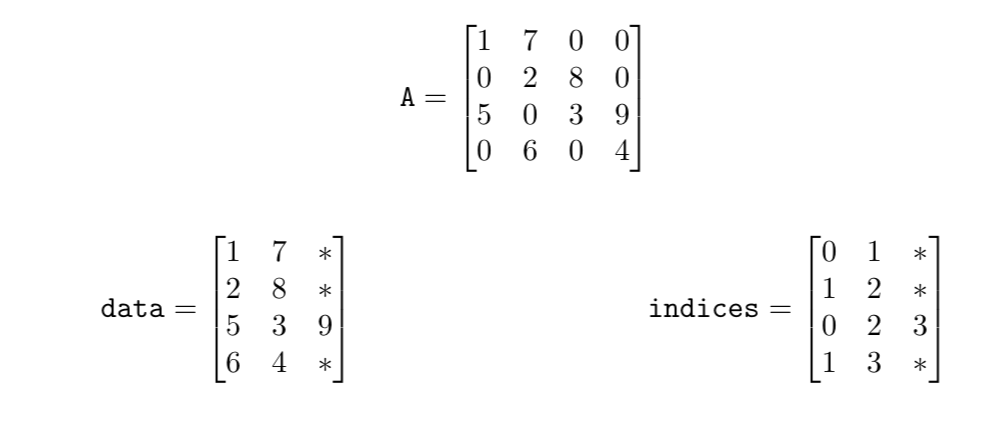
\includegraphics[width = 0.65\textwidth]{ellpack.png}
\end{figure}
For GPU computation, the method is the same as the Diagonal format, where each thread is assigned to a row and computes the dot-product, but instead using the index matrix as a hash for locations (and therefore accesses the index matrix continguously)

The performance of this relies on the fact that overall, most of the rows all have $Z$ elements (i.e. balanced numbers of elements on the rows), which load-balances the work performed on each thread.


\item Coordinate format - The most widely used and well known format being the CSR (compressed sparse row), the matrix $M$ is represented by ptr, indices, and data vectors which specify the offset on each row that has elements (with last element being the number of NNZ's), along with the distinct rows, and data elements, respectively. 
\begin{figure}[h]
  \caption{CSR example format}
  \centering 
  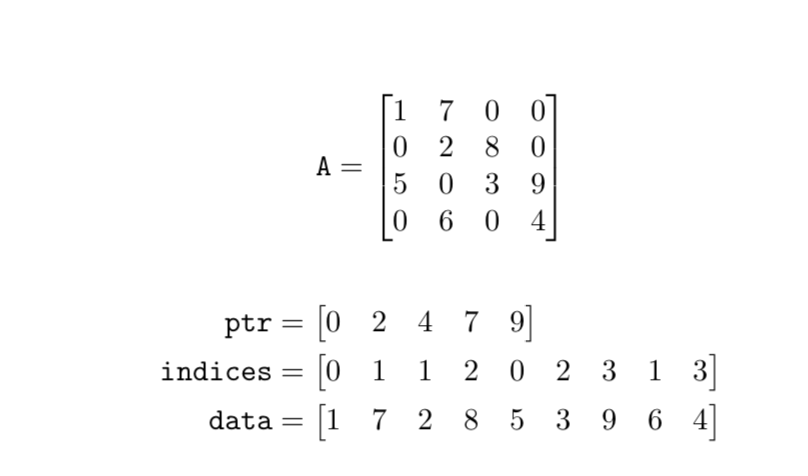
\includegraphics[width = 0.65\textwidth]{CSR.png}
\end{figure}
For the SpMV operation, the "vector kernel" is introduced, where an entire thread block may be assigned to each matrix row, whose entries are then partitioned equally among the threads, with a final parallel reduce operation to compute the dot product between the matrix row and vector. 
\end{itemize}




\subsection{SpMM}
In \cite{bell_spmm}, the algorithm is decomposed into 3 portions, assuming the input is $A, B$ and the output is $C = A \cdot B$. We also assume  $A,B$ are expressed in CSR (Compressed Sparse Row) format. The 3 portions are then the "expand, sort, compress" (ESC) methods, similar to a Map-Reduce technique, as explained below. 

\begin{figure}[h]
  \caption{Example of the 3 techniques, when $C$ is generated from $A,B$ which are in CSR format. }
  \centering 
  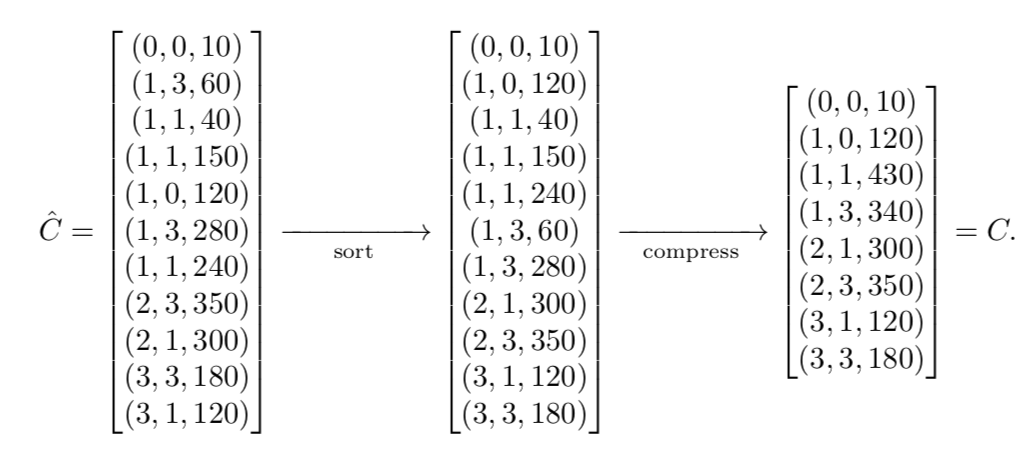
\includegraphics[width = 0.65\textwidth]{expand_sort_compress.png}
\end{figure}

\begin{itemize}
\item Expand: This generates all possible pairings $(A_{ik}, B_{kj})$ which are used to add to a position $C_{ij} += A_{ik}*B_{kj}$. The generation process can be viewed as forming all-pairs paths on a bipartite graph. More specifically, for a matrix $M$, the bottom side of the graph consists of vertices, each representing a row, while the top side's vertices represent the columns, with a connection (a,b) if the element $M_{ab}$ is non-zero. Then conjoining the bipartite graphs $A,B$ makes it convenient to see that the total number of pairings $(A_{ik}, B_{kj})$ is the number of length-2 paths. 

\begin{figure}[h]
  \caption{Example figure of expansion bipartite graphs}
  \centering 
  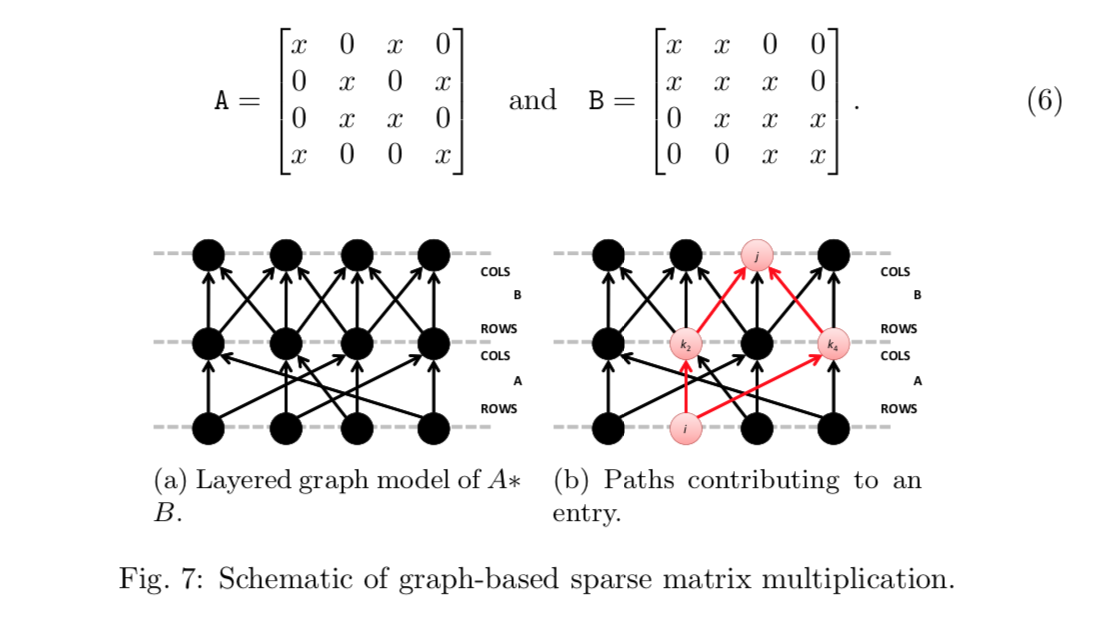
\includegraphics[width = 0.65\textwidth]{bipartite_MM.png}
\end{figure}
Thus, using out all length-2 paths corresponds to a "BFS"-type tracking on this path, from which well-known GPU graph traversal methods are used. In the GPU case, the best method would be for each thread to possess a starting node at the bottom side of the bipartite graph corresponding to $A$. A given core then selects $T$ consecutive bottom vertices, and the total vertices are partitioned by cores. Each thread $t$ then computes the "expansion" (i.e. all possible paths from its vertex $v_{t}$ including the products associated with a path), using techniques found in \cite{bfs_gpu}. 
\item Sort: This method sorts lexicographically each element $(x,y, c)$ generated from before, where $x,y$ corresponds to location $(x,y)$ in $C$, and $c$ is to be incremented to $C_{xy}$. This method is used to assist the compress portion, which is used to remove duplicate/increment $(x,y)$ coordinate entries. Sorting is cited as the most computationally expensive configuration, and the algorithm to invoke derives from the work \cite{sort}. The baseline algorithm is an inspired GPU-based Radix Sort, found in Thrust's \code{stable\_sort\_by\_key} algorithm. Here, the number of threads is proportional to the number of elements in the expansion, and the total elements is partitioned equally for each thread, (over same rows) with each thread sorting only its sub partition. All of the sorted sub partitions are then collected within the block shared memory, and then re-sorted within the entire block, which sorts an entire row.  



\item Compress: This section invokes the work found in \cite{multigrid}, and calls the Thrust function \code{reduce\_by\_key} algorithm, which for each row index $i$, the function collects all entries positioned in row $i$. The algorithm then performs "reduction" (i.e. combine consecutive terms with the same $j$ index) and outputs the compressed format. However, since it is not known at runtime which positions (i,j) have very large duplicate entries, it would be highly inefficient to assign each thread to a position (i,j) on the GPU. Instead, a scan is implemented at first to check which duplicate positions exist, and then partitions all duplicate entries into consecutive, fixed-length blocks for each thread to reduce, attempting to load balance. 
\end{itemize}



\section{Experiments}

\subsection{Code}
Our code and scripts can be found on:

\url{https://github.com/Srizzle/GPU-Sparse-Matrix-Multiply-CS-267}. The scripts used for simulation are: 
\begin{itemize}
\item CUSP: cusp.cu - \url{https://github.com/Srizzle/GPU-Sparse-Matrix-Multiply-CS-267/blob/master/cusp.cu}
\item CUPY: cupy.py - \url{https://github.com/Srizzle/GPU-Sparse-Matrix-Multiply-CS-267/blob/master/cupy_script.py}
\item Pyculib: pyculib\_script.py - \url{https://github.com/Srizzle/GPU-Sparse-Matrix-Multiply-CS-267/blob/master/pyculib_script.py}
\item CPU: cpu\_script.py - \url{https://github.com/Srizzle/GPU-Sparse-Matrix-Multiply-CS-267/blob/master/cpu_script.py}
\end{itemize}


\subsection{Hardware}
We applied our experiments on the following hardware specified on Amazon AWS:
\begin{itemize}
\item Nvidia Tesla K80 
\item 11.75 ECUs, 4 vCPUs, 2.7 GHz, Intel Broadwell E5-2686v4, 61 GiB memory, EBS only, with Intel AVX and Turbo allowed. 
\end{itemize}
Note that for this case of GPU, the memory bandwith is relatively larger than other GPU's of similar costs (480 GB/s vs 288 GB/s on a Tesla K40) 

\subsection{Erdos Reynii}
We at first tested multiplication for $N \times N$ matrices, where each element was non-zero with probability $p$, where: 
\begin{itemize} \item $N \in \{2^{4},...,2^{14} \}$ \item $p \in \{0.01, 0.02, 0.03, 0.04, 0.05, 0.1, 0.15, 0.2, 0.25, 0.3, 0.35, 0.4, 0.45, 0.5\}$
\end{itemize}
Note that for floats (where a float32 is a byte), when $N = 2^{14}$, $p = 0.01$, $pN^{2} \text{(float size = 1 byte)} \approx 2 GB$, and at $N = 2^{14}, p = 0.5$, $pN^{2} \cdot \text{(float size = 1 byte)} = 134 GB$. Since the K80 RAM has 24GB of memory, this is reaches the order-magnitude of the GPU memory (i.e. for $N = 2^{15}$ sizes and higher, memory hardware limits are broken and disallowed at runtime). 



\subsection{Real World Data}
Real world data matrices were also used in computation, found in \url{https://sparse.tamu.edu/}. We found the matrices that best fit the parameter (e.g. closest to a given sparsity $p$ and size $N$) The matrices used were: 
\begin{figure}[h]
  \caption{Real World Graph Names}
  \centering 
  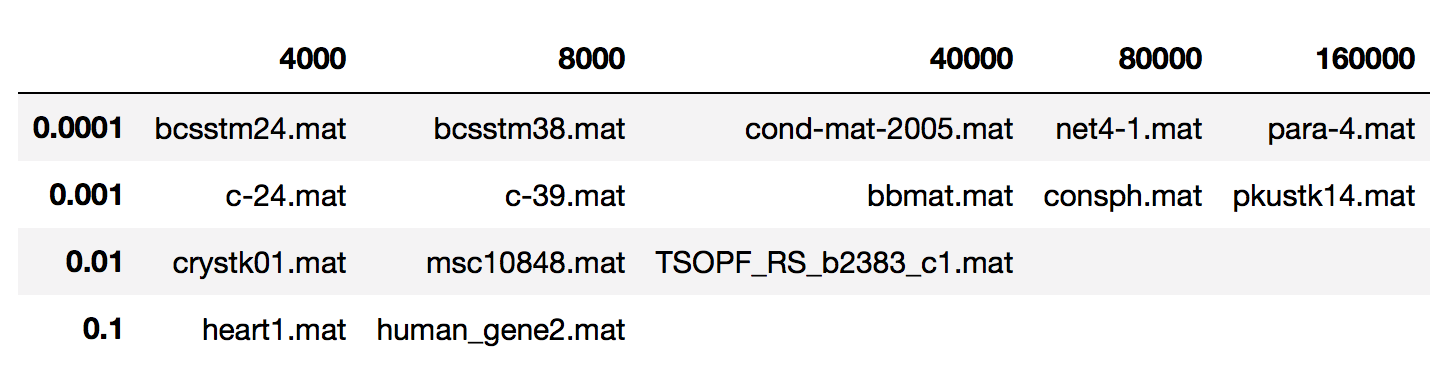
\includegraphics[width = 0.8\textwidth]{matrix_names.png}
\end{figure}

\newpage 

\section{Performance and Results}


\subsection{Erdos Reynii}
The results for the Erdos Reynii model were completely out of expectation - for instance, cuBLAS did not increase in time complexity as we varied the size of the matrix - this is due to the fact that purely random matrices do not allow libraries to exploit their structure. Thus, we will not sketch those results in this report. However, we encourage the reader to see the results found in \url{https://github.com/Srizzle/GPU-Sparse-Matrix-Multiply-CS-267/tree/master/Erdos_Reynii_Experiments}. We saw from these experiments that cuBLAS did not show an increase in runtime regardless of $N = 2^{14}$ or $N = 2^{5}$, while cuSPARSE ran significantly slower as well. 

\subsection{Real World Data}
We have the following colors over all graphs -  
(Purple: CUSP, Red: CuSPARSE, Blue: cuBLAS). The graphs can be found in the Appendix ~\ref{appendix}.

\begin{comment}
\subsubsection{cuBLAS (CuPY)}
\begin{figure}[h]
  \caption{Performance for cuBLAS (in order, CSR $\times$ CSR, CSR $\times$ DenseMatrix, CSR $\times$ DenseVector}
  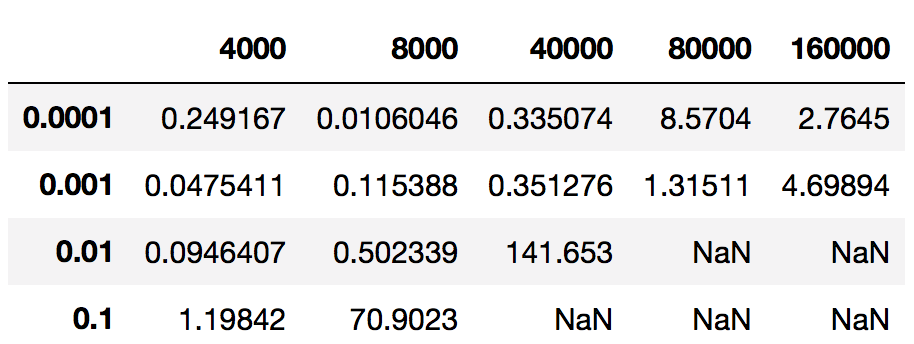
\includegraphics[scale = 0.24]{csr_x_csr_cublas.png}
  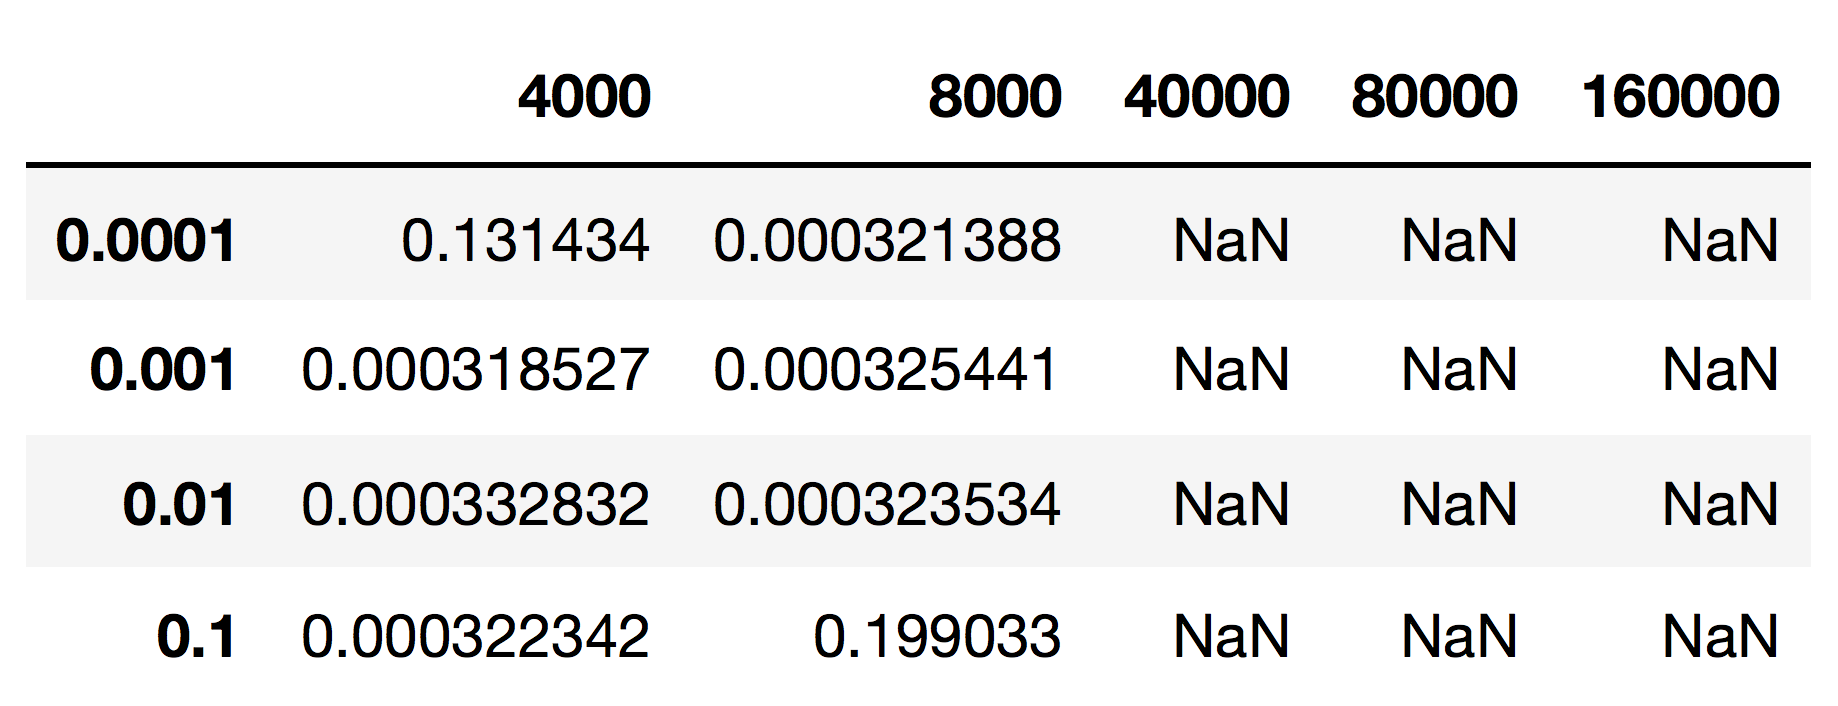
\includegraphics[scale = 0.25]{csr_x_densematrix_cublas.png}
  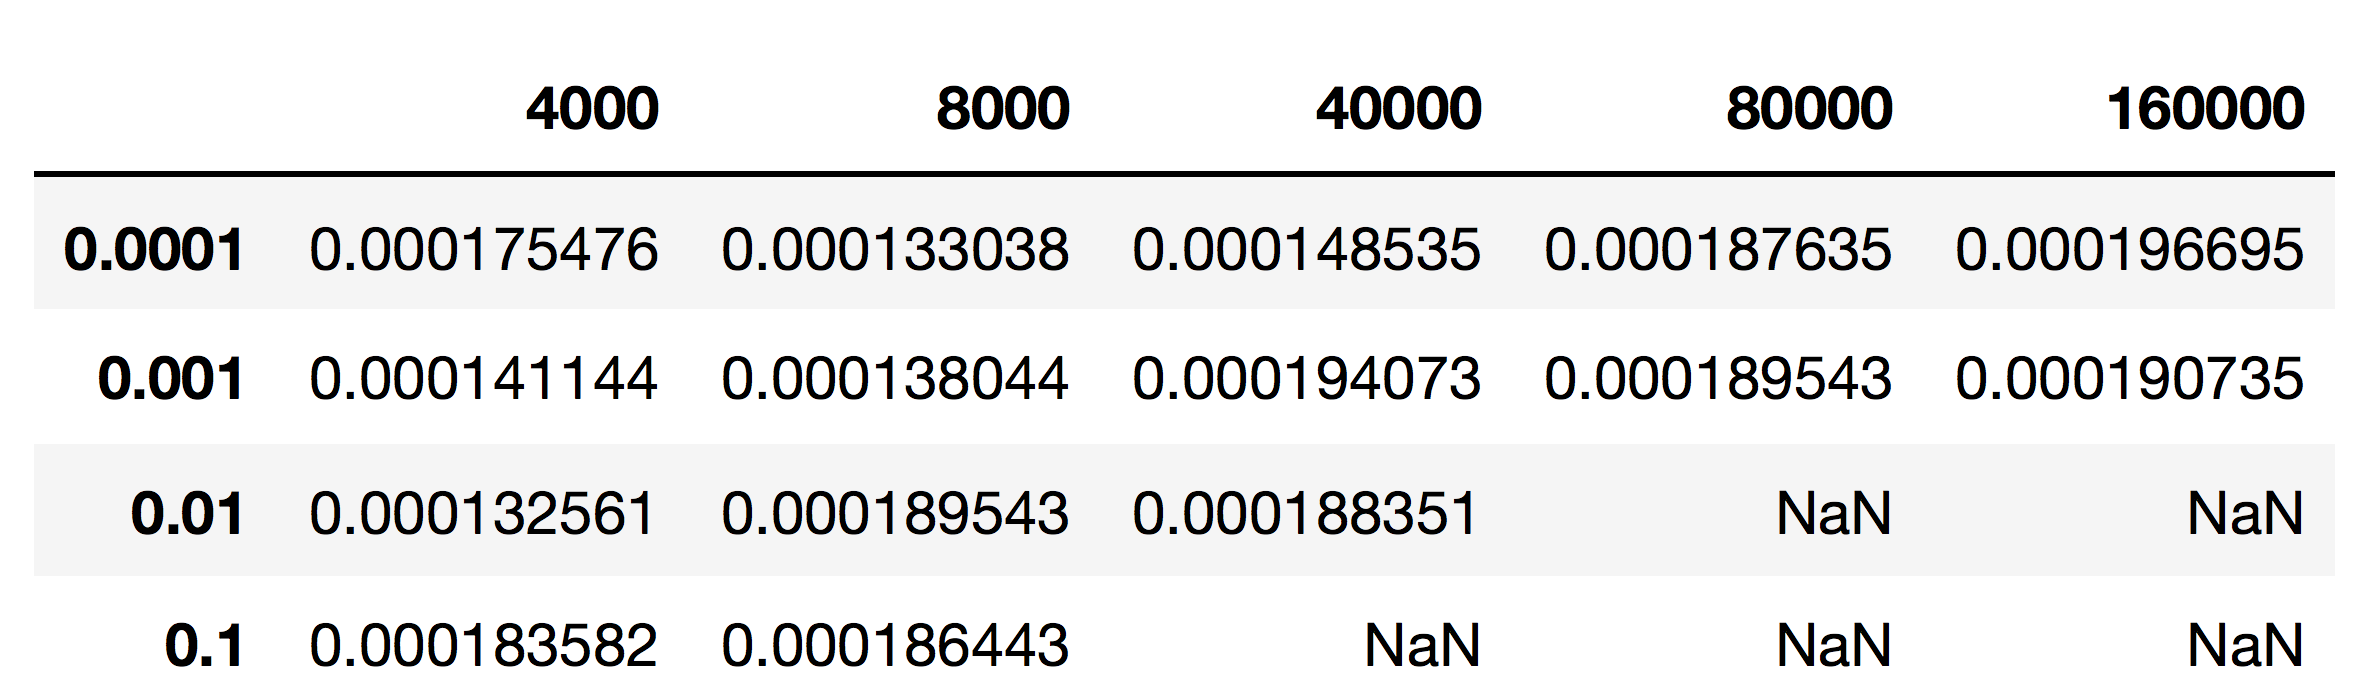
\includegraphics[scale = 0.23]{csr_x_densevector_cublas.png}
\end{figure}

\subsubsection{cuSPARSE (PyCuLib)} 
\begin{figure}[h]
  \caption{Performance for cuSPARSE (in order, CSR $\times$ CSR, CSR $\times$ DenseMatrix, CSR $\times$ DenseVector}
  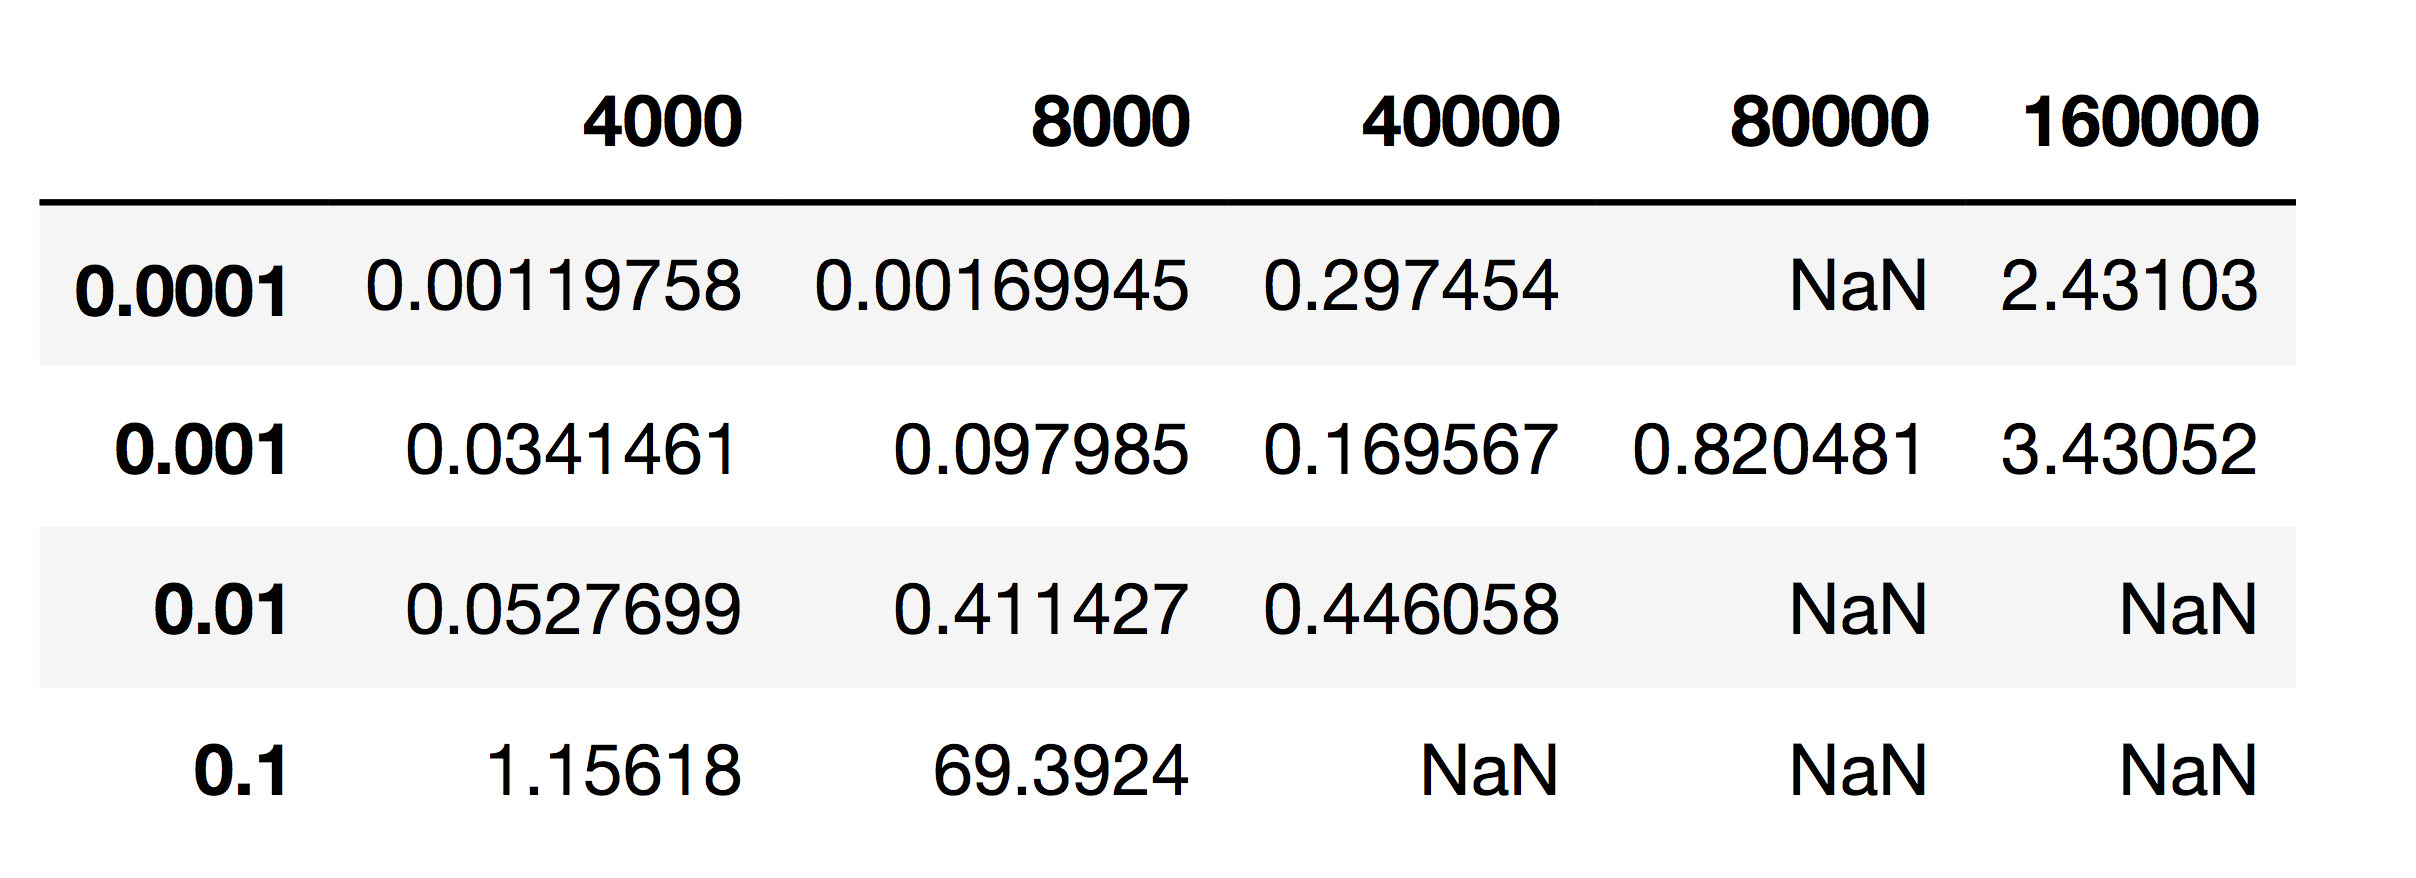
\includegraphics[scale = 0.20]{csr_x_csr_cusparse.png}
  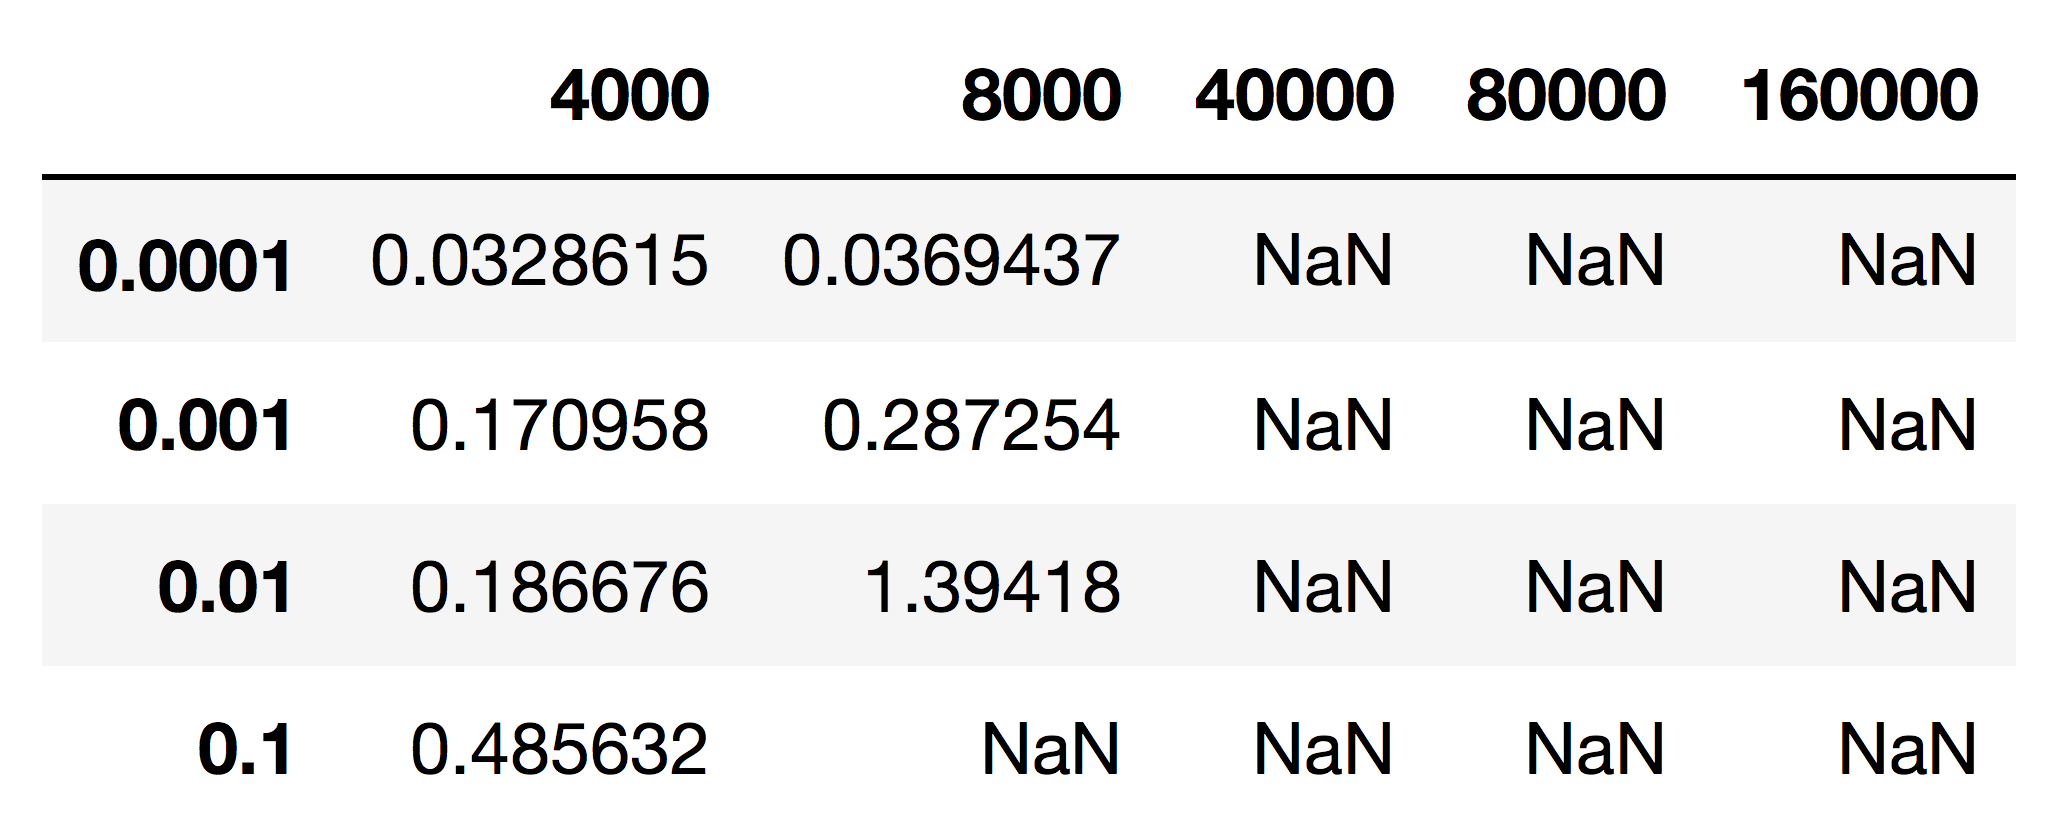
\includegraphics[scale = 0.22]{csr_x_densematrix_cusparse.png}
  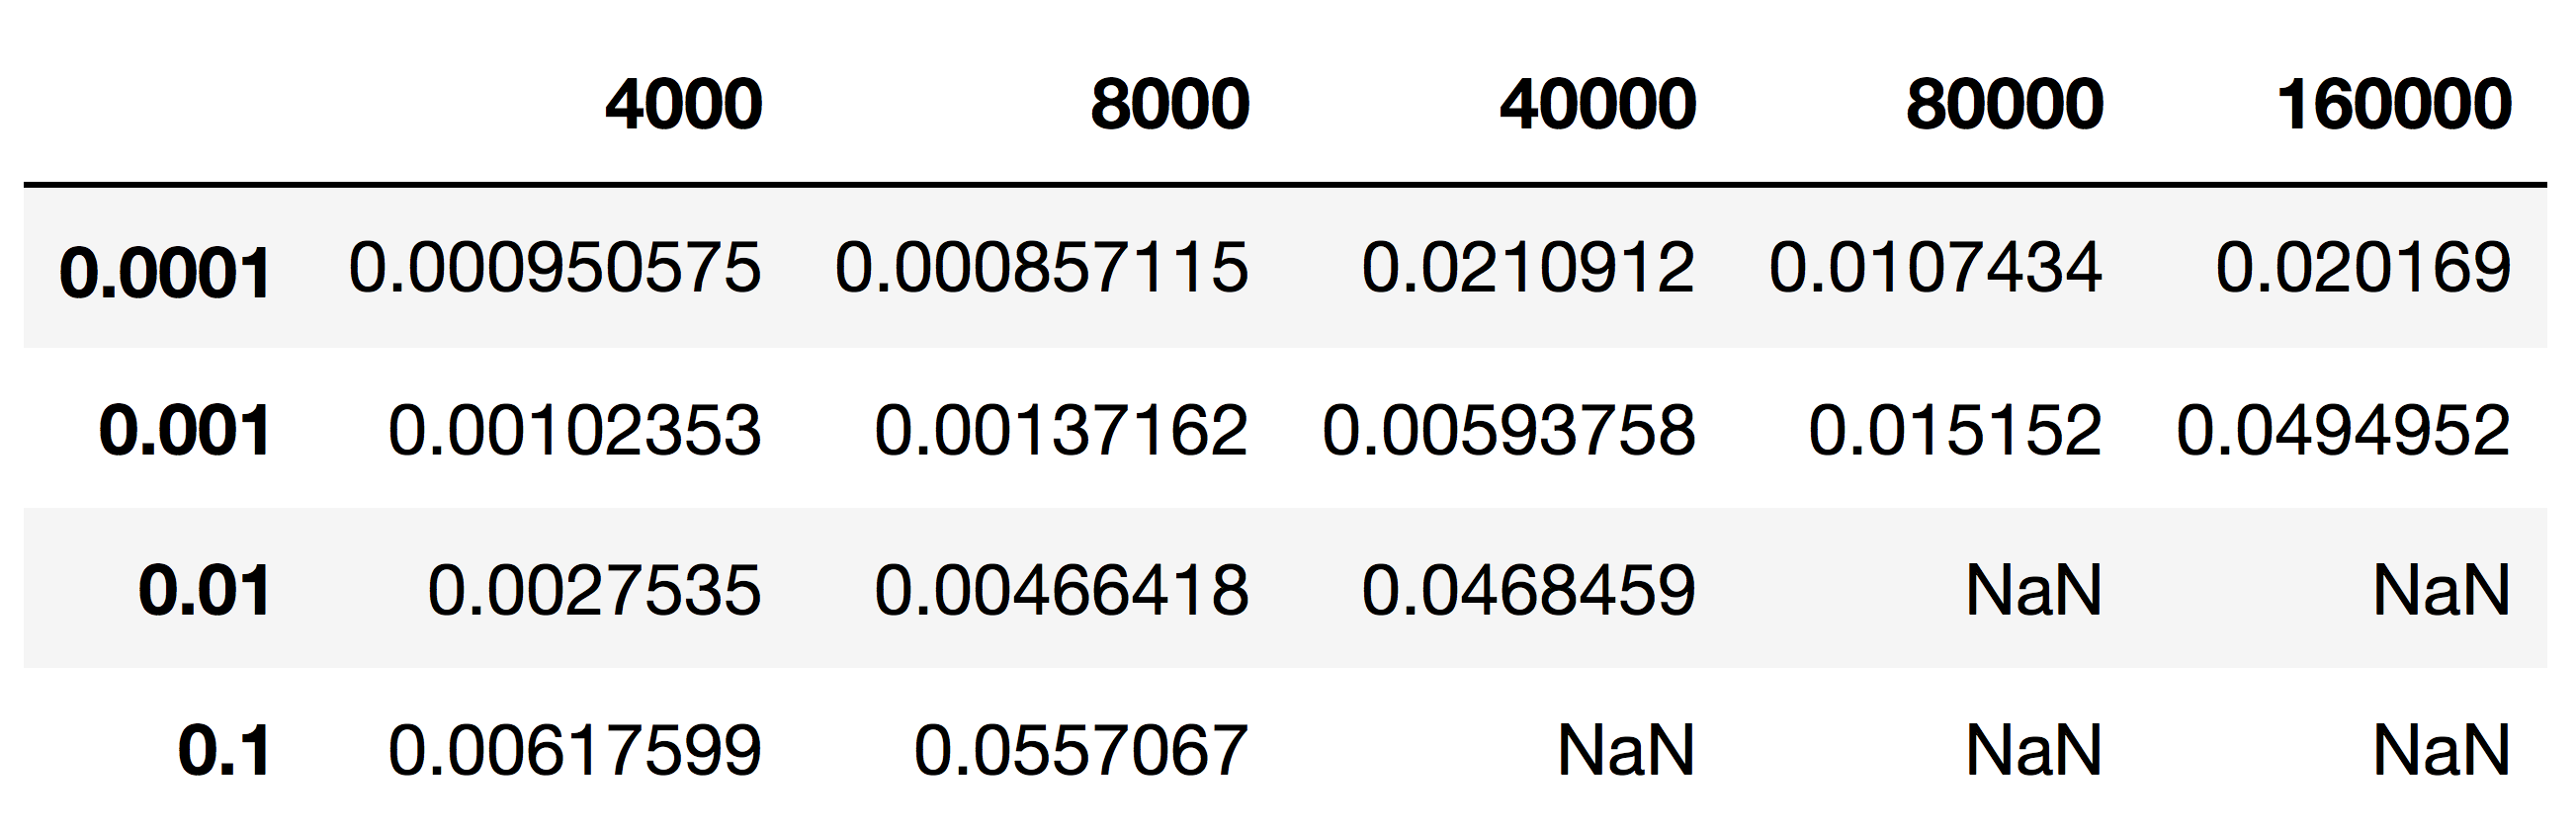
\includegraphics[scale = 0.22]{csr_x_densevector_cusparse.png}
\end{figure}
\newpage 
\end{comment}
\subsection{Analysis}
From the data, the most interesting trend was generated by CSR x CSR. We see that cuSPARSE did perform better than CUSP in some particular areas (CSR x CSR at p = 0.001, or CSR x DenseVector early on), but did not outperform cuBLAS in any of the experiments, although was very close in small matrix sizes. Furthermore, we also see that at higher densities, cuSPARSE did indeed increase the most, as expected. cuBLAS had a slow increase in some parts. 

For other cases (CSR $\times$ DenseVector or CSR $\times$ Dense Matrix), as expected, cuBLAS remained the most efficient (due to the dense portions)

In terms of runtime, note that for very sparse matrices ($p = 0.0001$), the general trend for all algorithms seems to be sublinear. However, as we increase the density, we can see a convex curvature, as well as suggesting a quadratic runtime. This is due to the fact that increased density eventually forces the NNZ number not to approximate $O(n)$, but towards $O(n^{2})$, which is unacceptable and not intended for sparse multiplication. 

\section{Further Work}
There is a variety of further directions that we wished to pursue, but in the interest of time, we did not. 
\subsection{Measuring Components}
It would be interesting to measure the performance of e.g. the separate expansion, sort, and compress algorithms in SpMM, to verify the claimed higher runtime of the sorting section.

\subsection{Memory Latency}
Because different GPU architectures possess very different memory-load bandwidths, this suggests further testing for different GPUs (K80, P100, etc.) which may affect performance. There have been other variants of GPU matrix algorithms, found in 

\subsection{Expanding Memory}
The size of the GPU RAM restricted our experiment sizes, as any larger dimensions would have overloaded the GPU RAM. Normally, the solutions to this type of problem either feature: 1. Use different GPU's with higher RAM 2. Distribute memory and workload across multiple GPU's.

\subsection{Different Matrix Shapes}
Note that from well known results in random matrix theory, a Erdos-Reynii matrix can have high probability of being singular \cite{singular}. Furthermore, the Erdos-Reynii format is generally not realistic, with many matrices in real world applications having generally high block sparsity. While we tested performance on widely used datasets, we did not use the other special sparse matrix formats (e.g. COO, ELLPACK, etc.), which may affect performance as well.   


\newpage

\bibliographystyle{alpha}
\bibliography{bib1}

\section{Appendix} \label{appendix}

\newpage 

\begin{figure}[h]
  \caption{CSR $\times$ CSR performance (first 4), then CSR $\times$ Dense performance (next 2), then CSR $\times$ DenseVector performance (last 4) }
  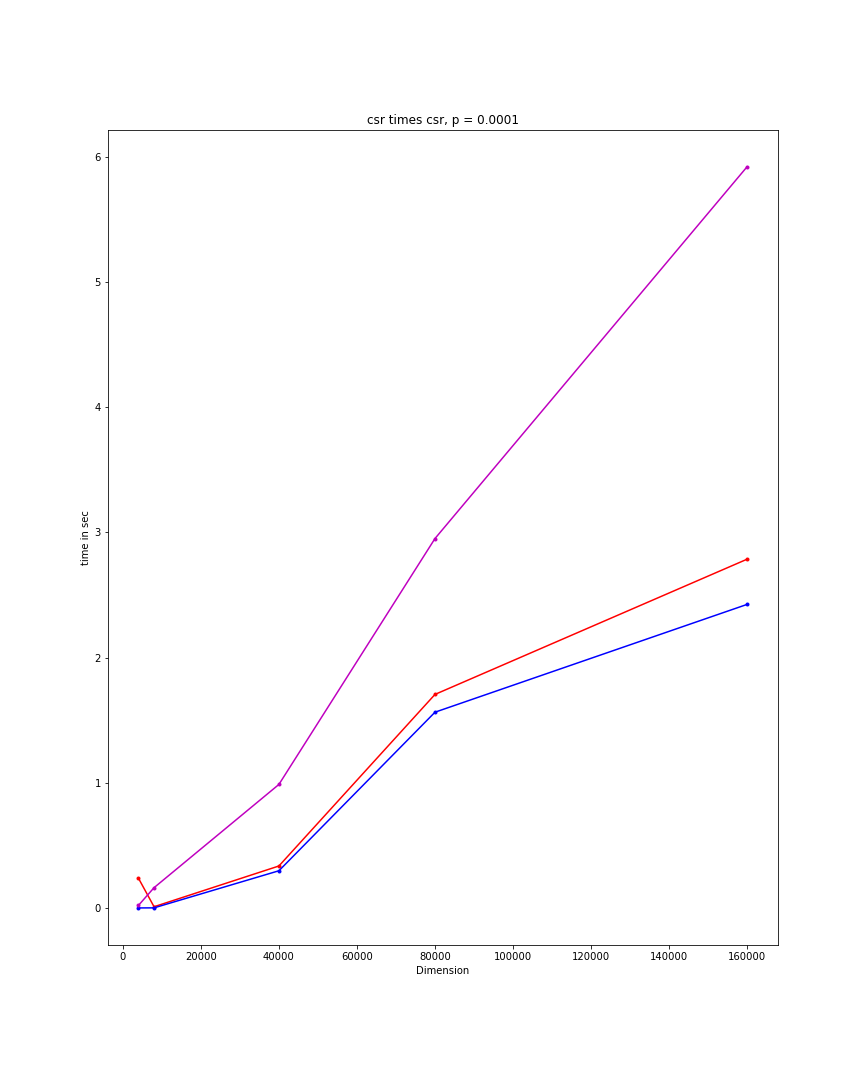
\includegraphics[scale = 0.16]{csr_csr_0001.PNG}
  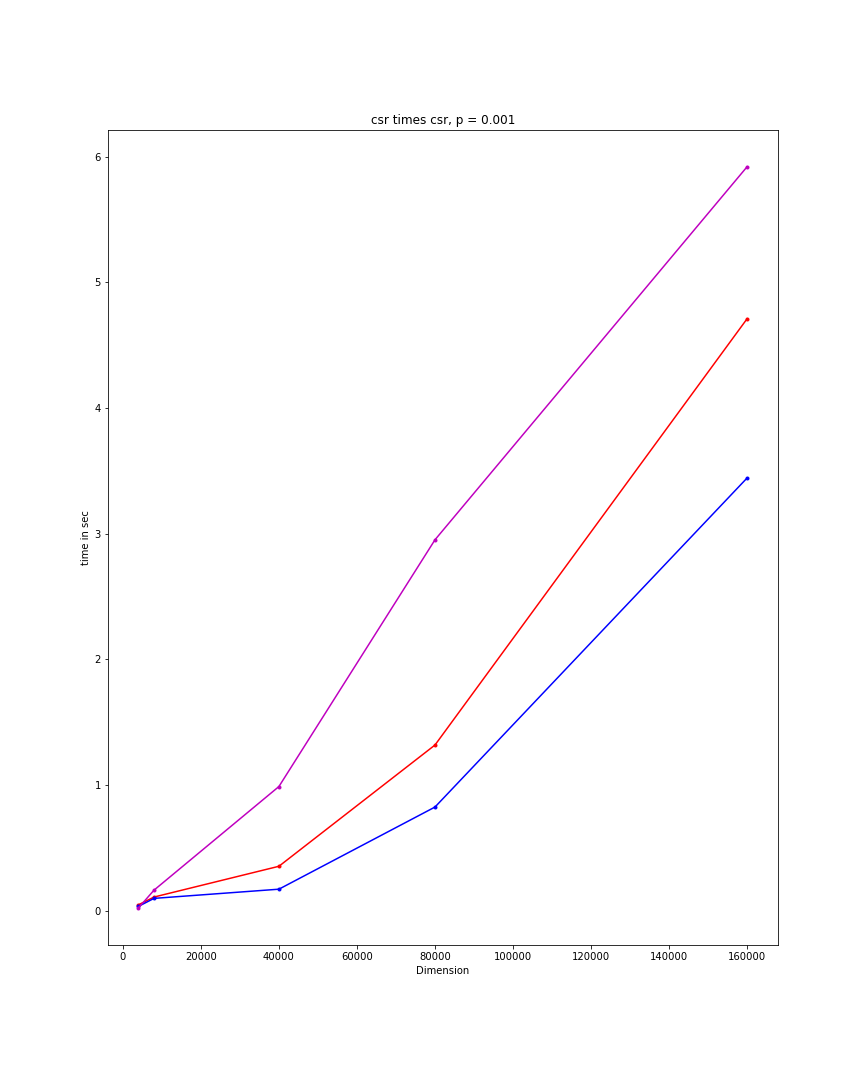
\includegraphics[scale = 0.16]{csr_csr_001.PNG}
  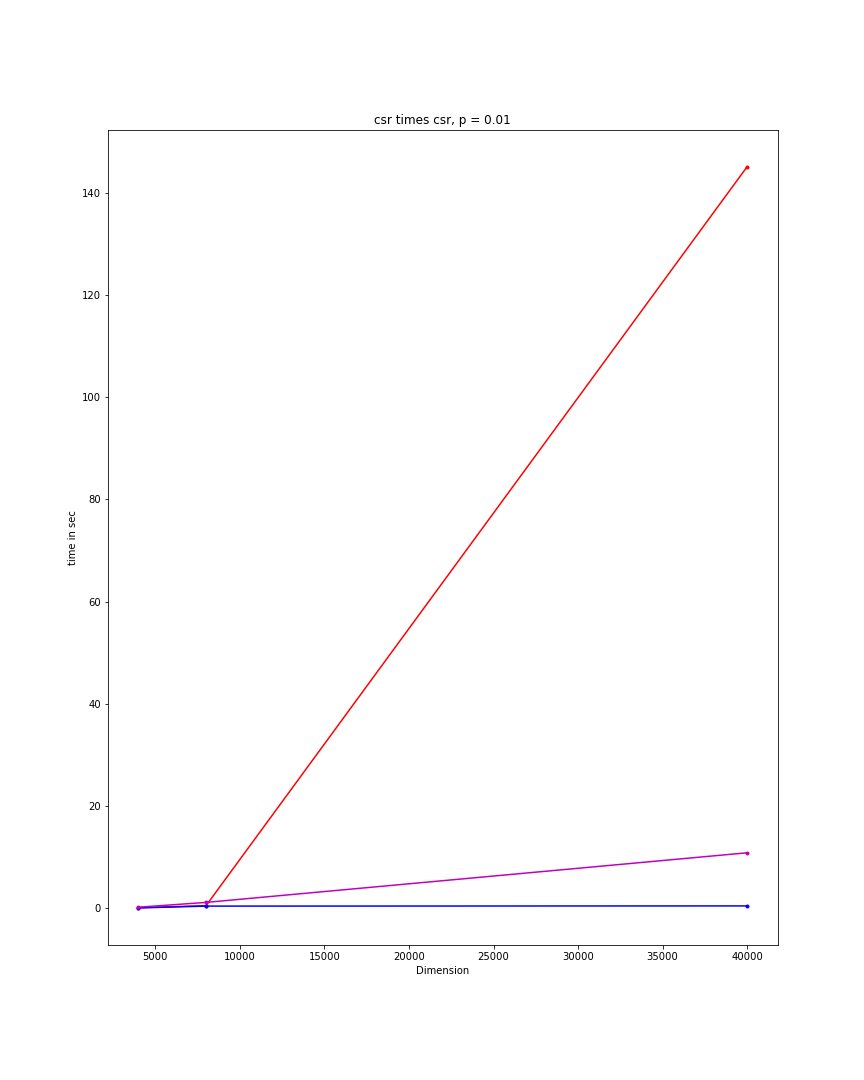
\includegraphics[scale = 0.16]{csr_csr_01.PNG}
  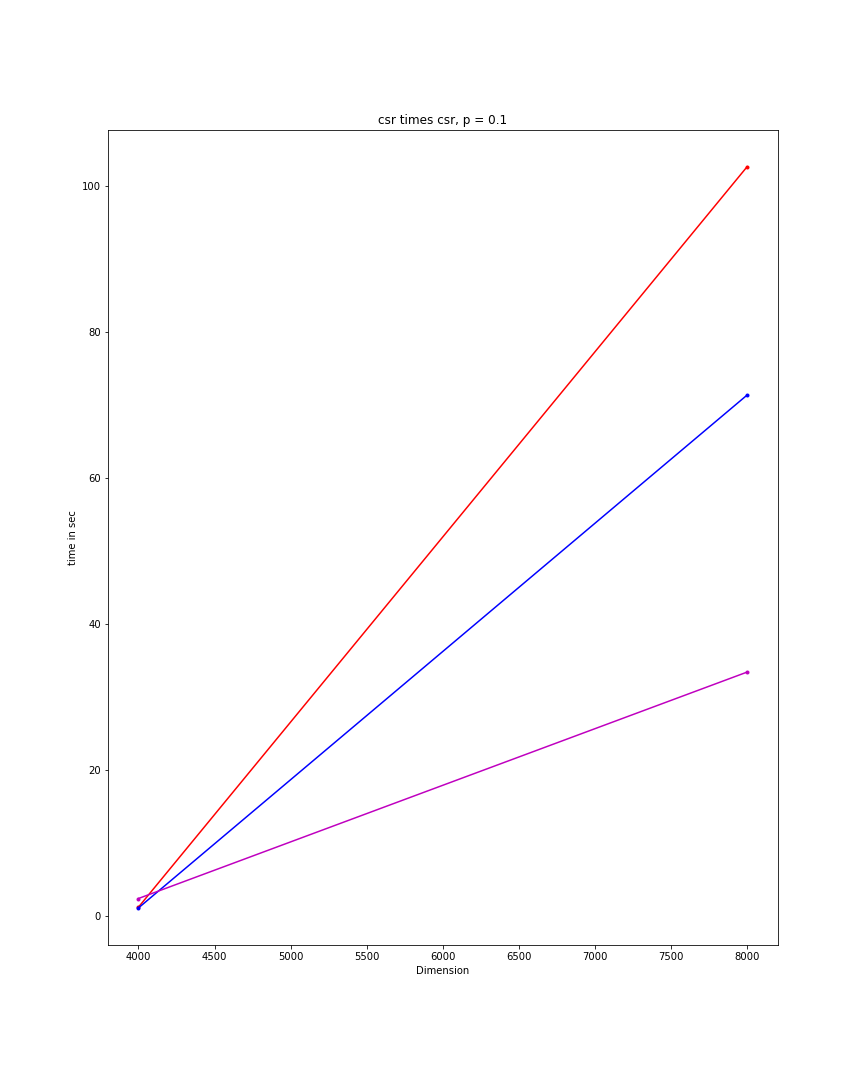
\includegraphics[scale = 0.16]{csr_csr_1.PNG}
  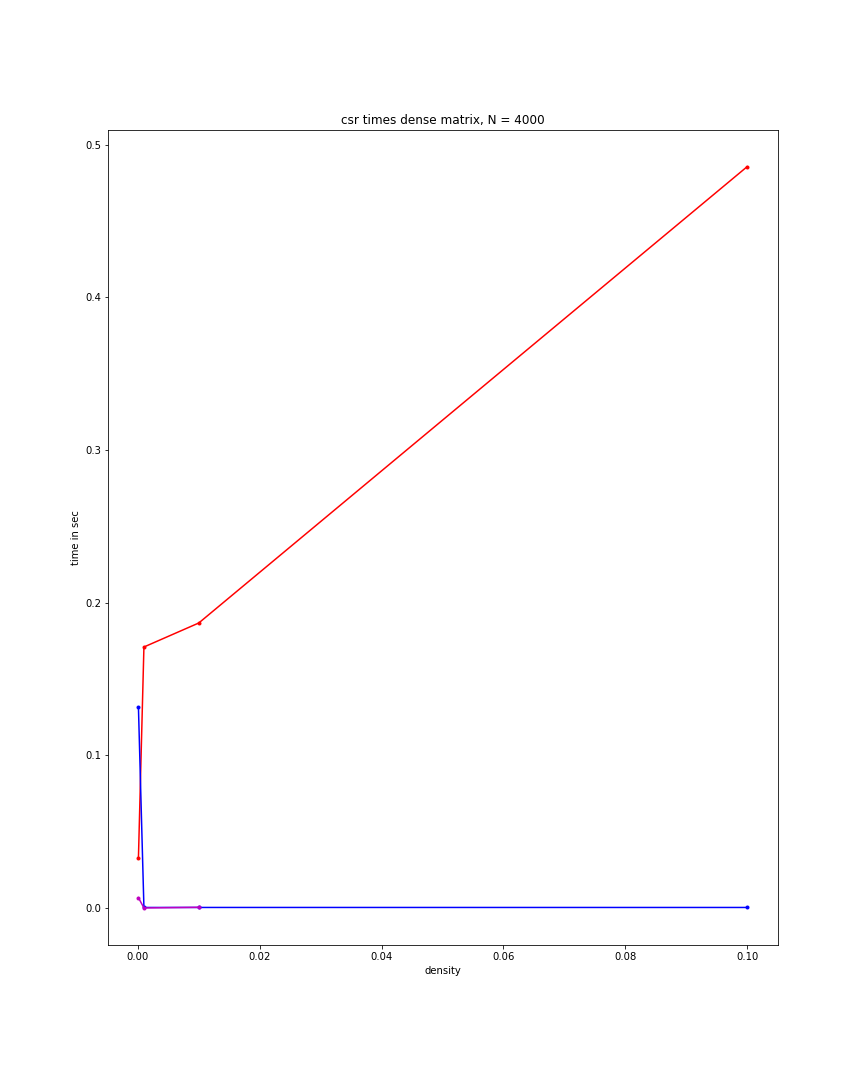
\includegraphics[scale = 0.16]{csr_dm_4000.png}
  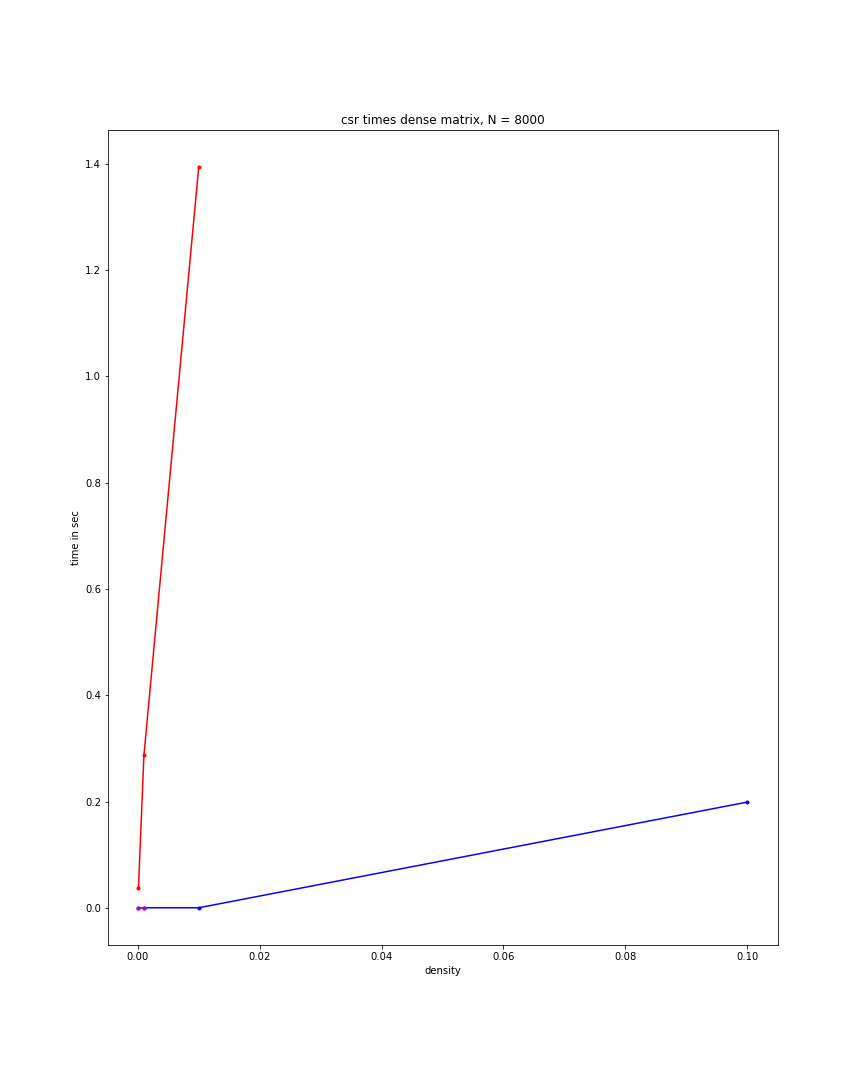
\includegraphics[scale = 0.16]{csr_dm_8000.png}
  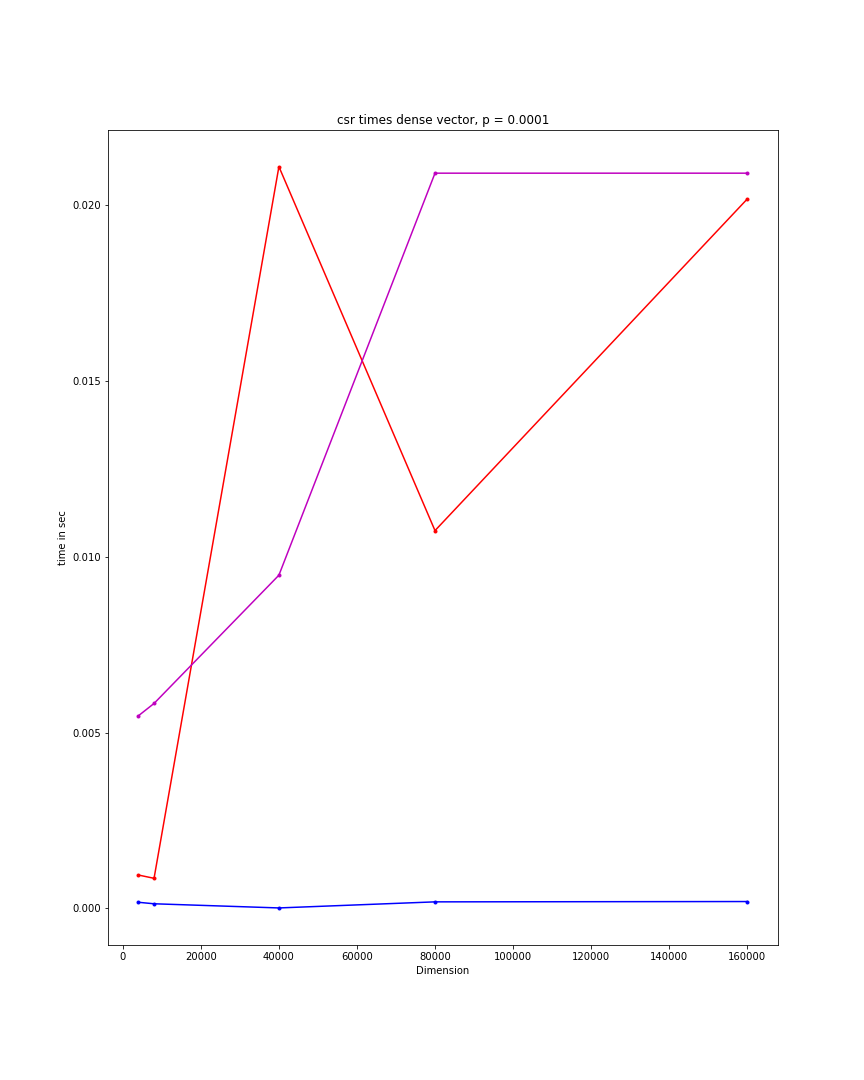
\includegraphics[scale = 0.16]{csr_dv_0001.png}
  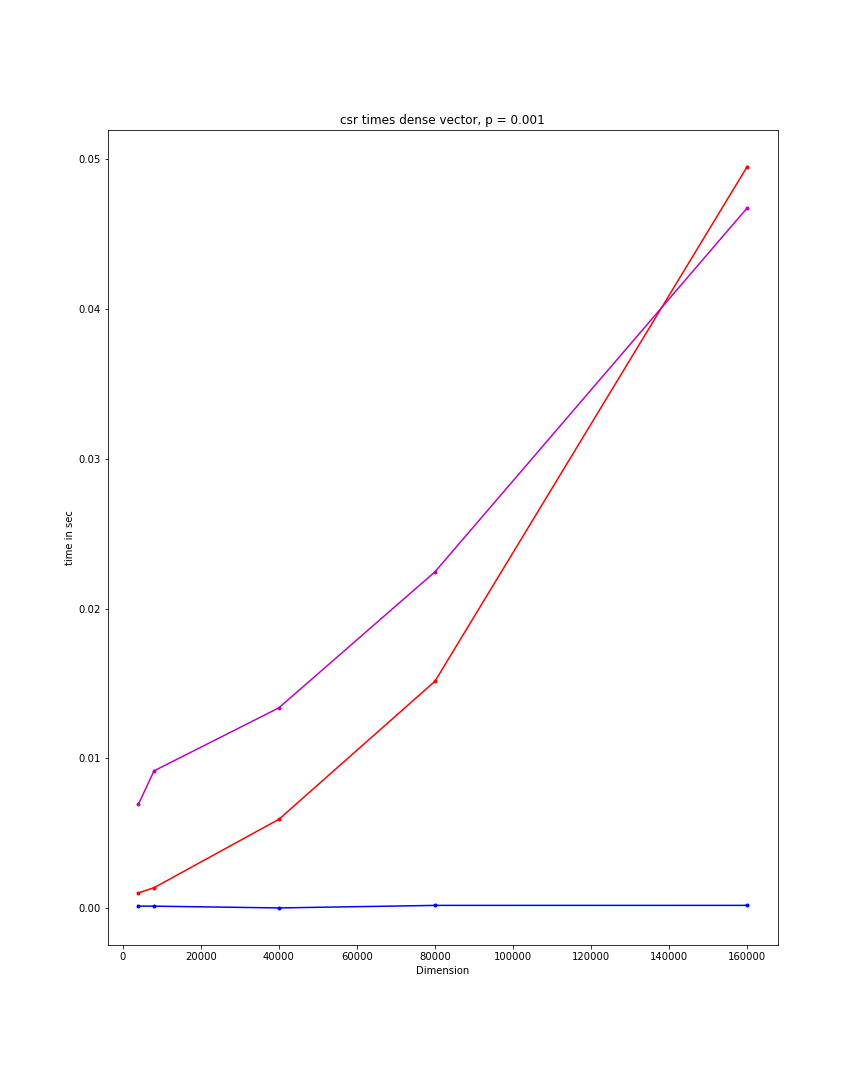
\includegraphics[scale = 0.16]{csr_dv_001.png}
  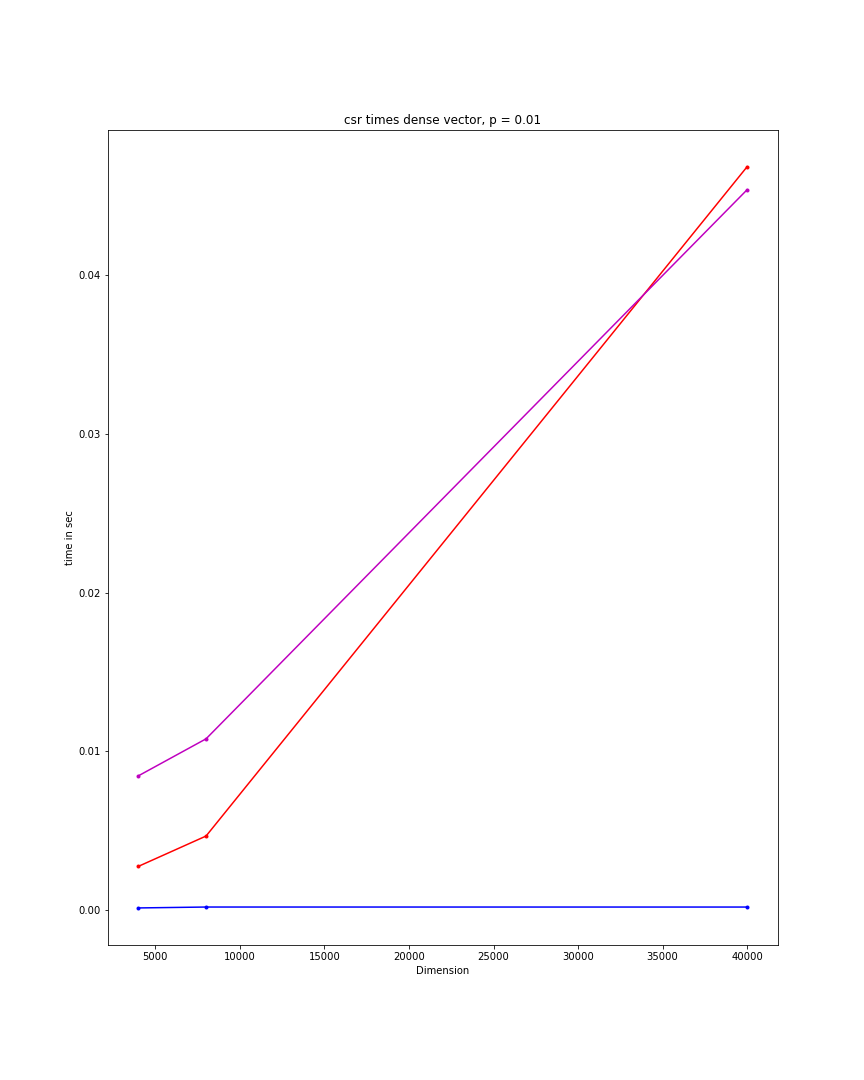
\includegraphics[scale = 0.16]{csr_dv_01.png}
  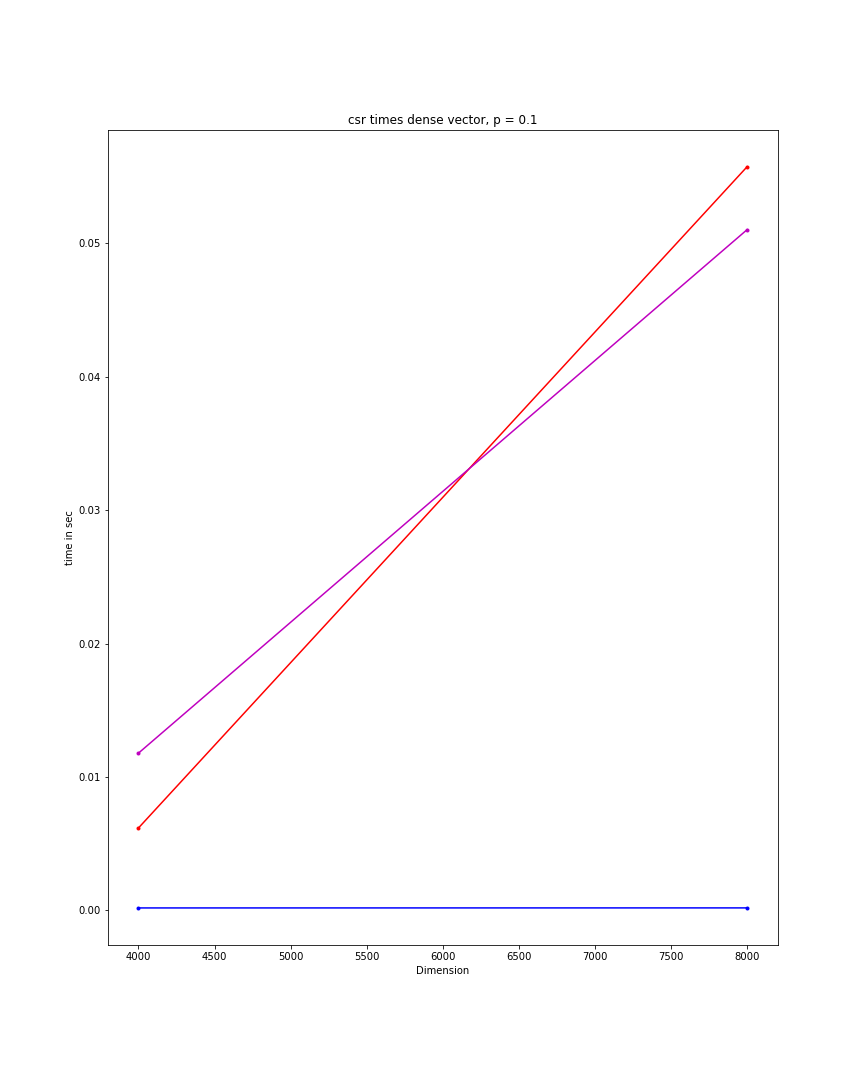
\includegraphics[scale = 0.16]{csr_dv_1.png}
\end{figure}



\begin{figure}[h]
  \caption{Log graphs of the previous results.}
  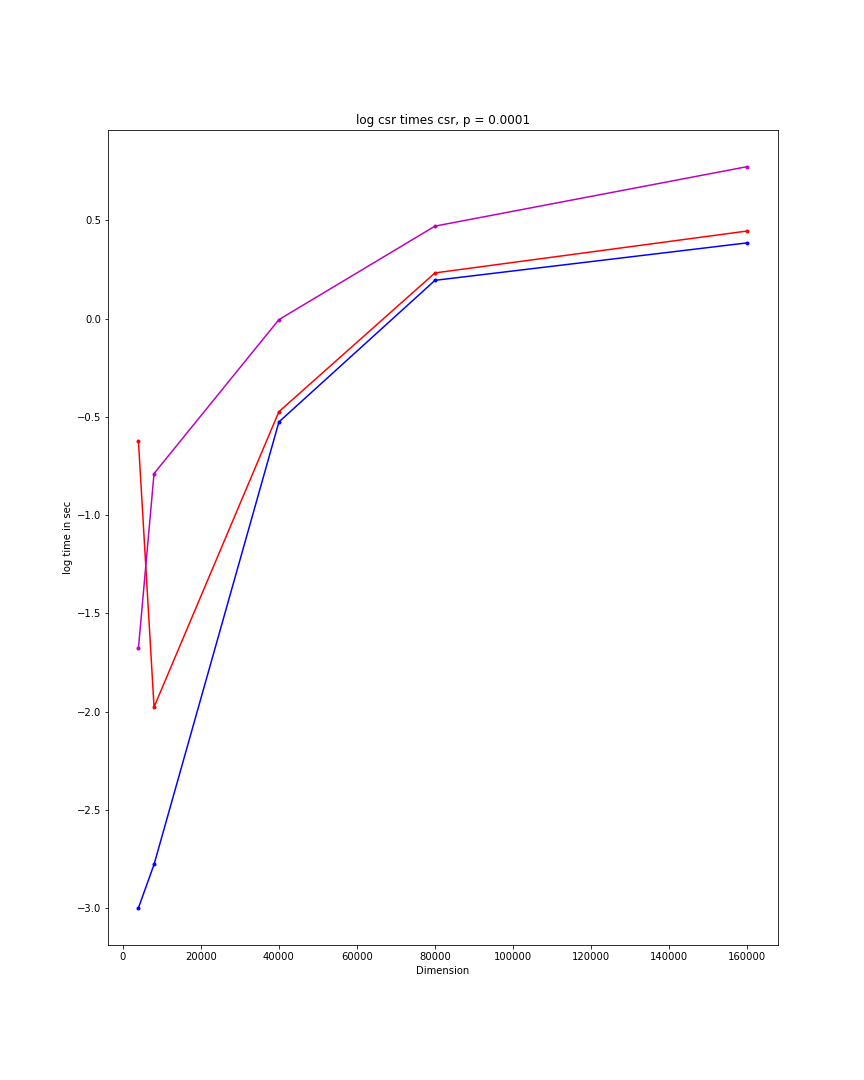
\includegraphics[scale = 0.16]{log_csr_csr_0001.PNG}
  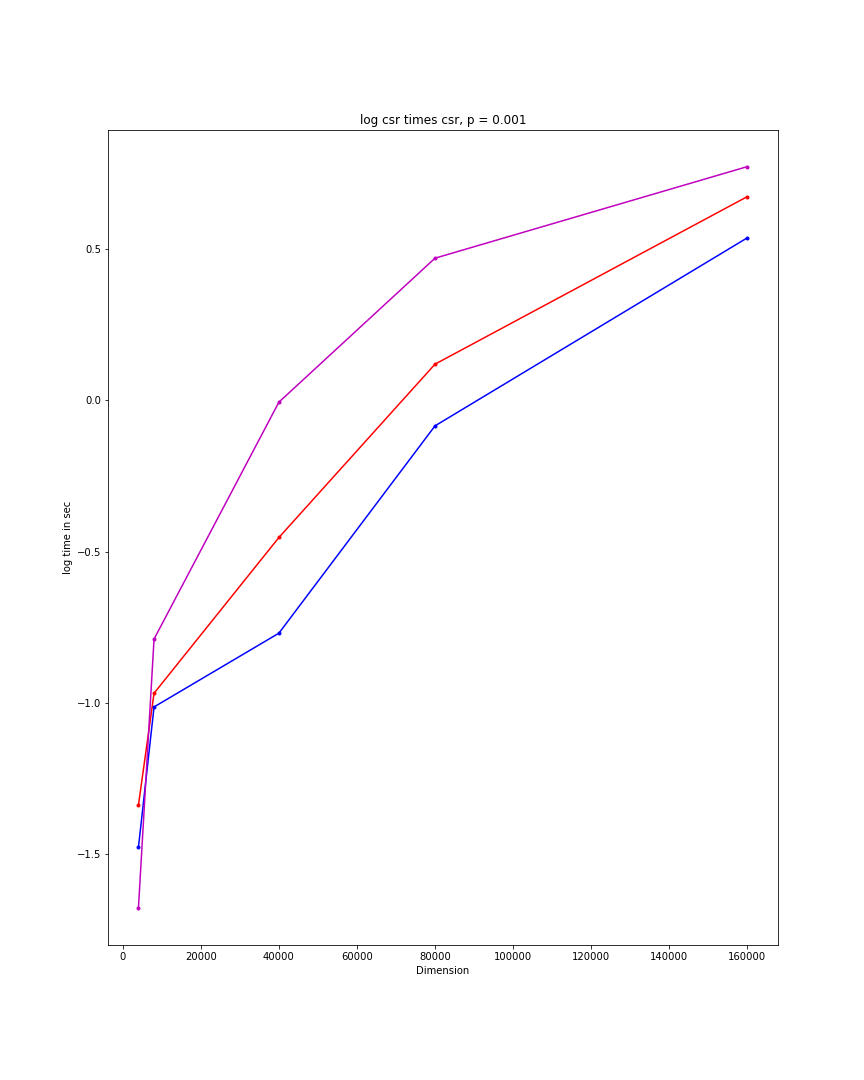
\includegraphics[scale = 0.16]{log_csr_csr_001.PNG}
  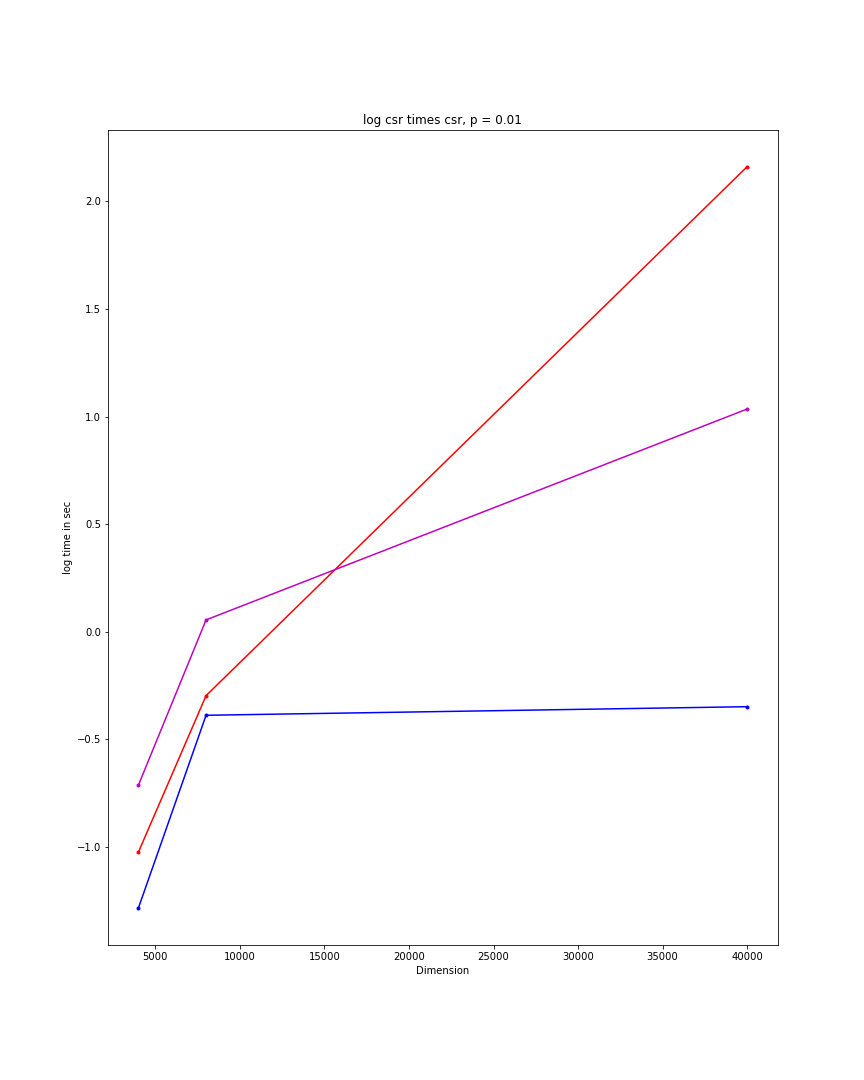
\includegraphics[scale = 0.16]{log_csr_csr_01.PNG}
  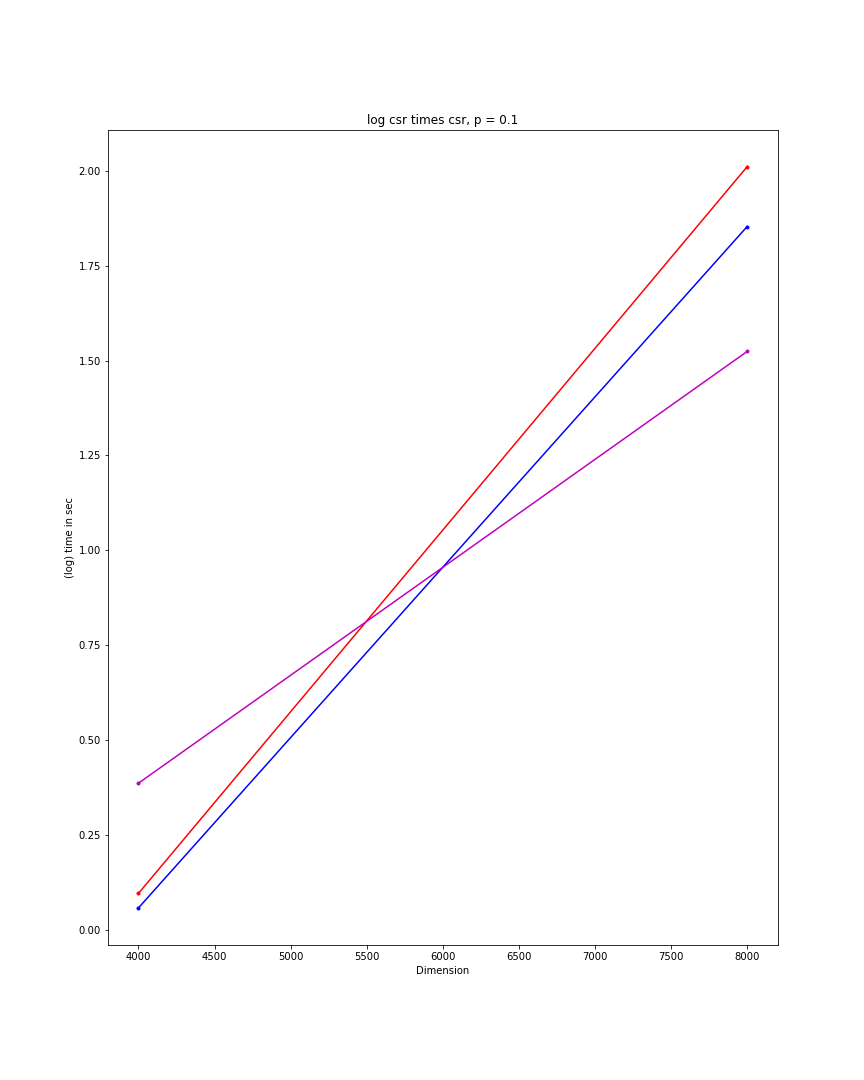
\includegraphics[scale = 0.16]{log_csr_csr_1.PNG}
  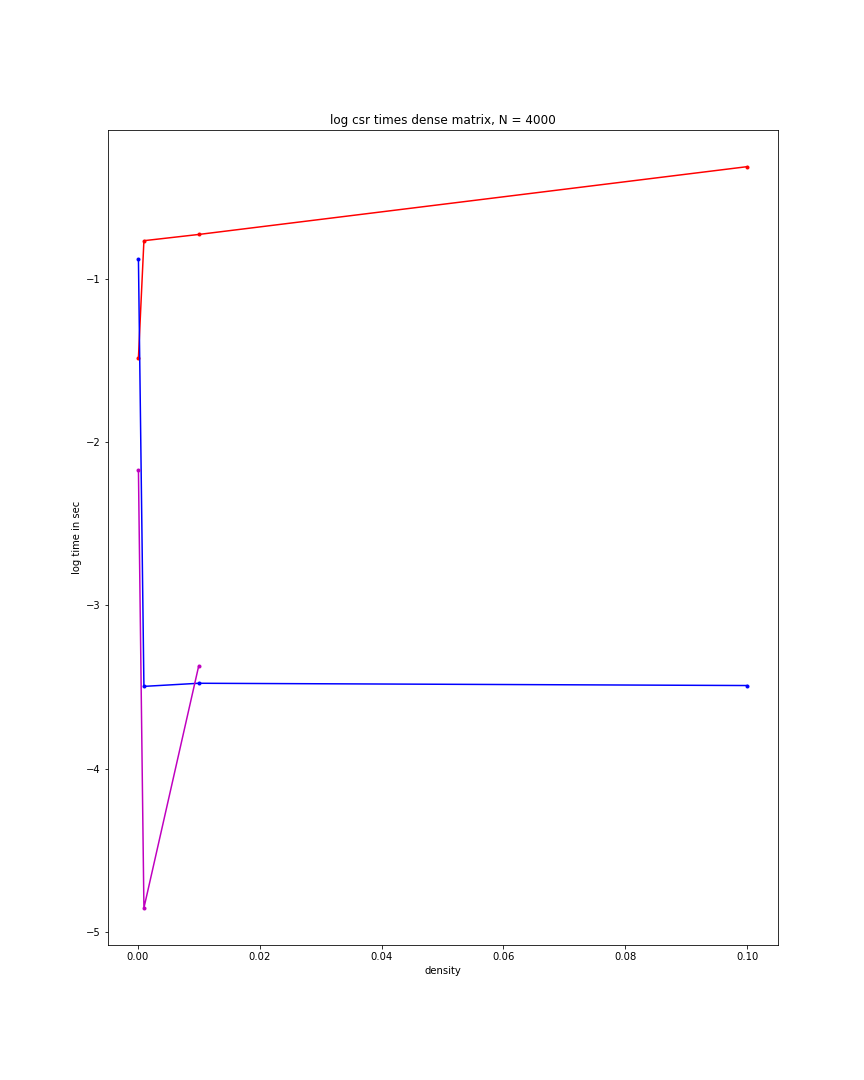
\includegraphics[scale = 0.16]{log_csr_dm_4000.png}
  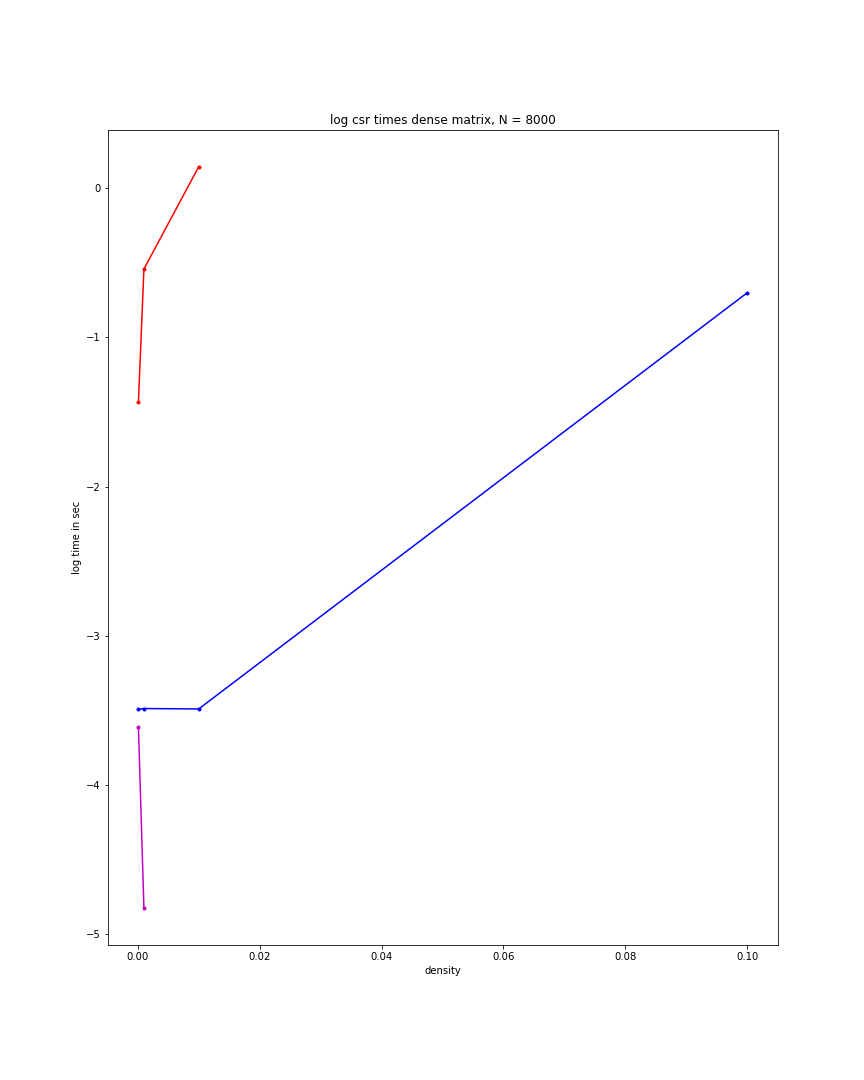
\includegraphics[scale = 0.16]{log_csr_dm_8000.png}
  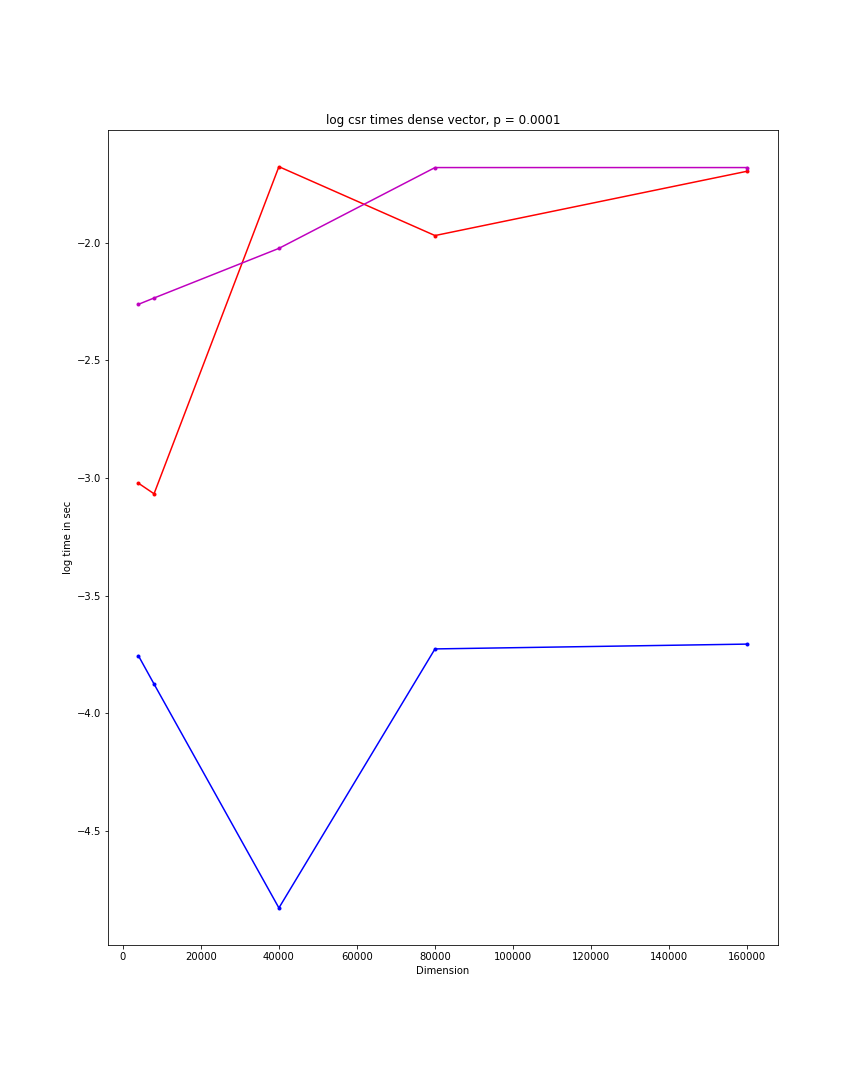
\includegraphics[scale = 0.16]{log_csr_dv_0001.png}
  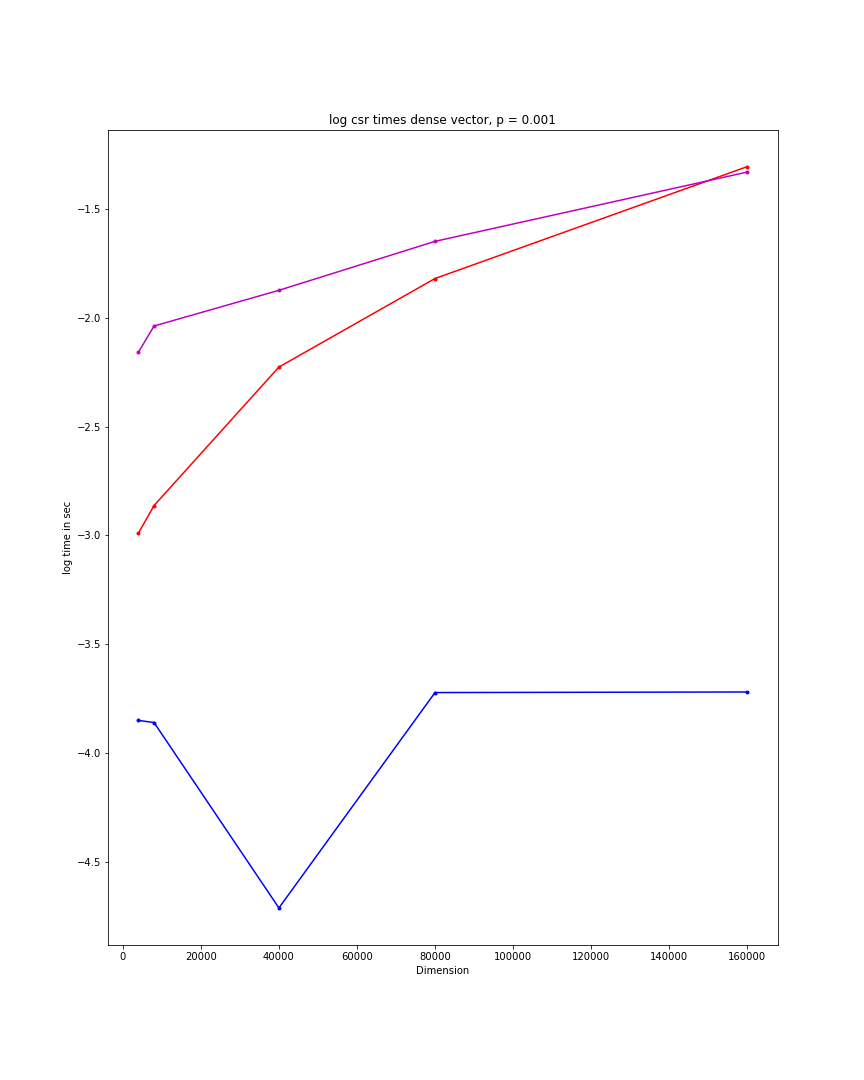
\includegraphics[scale = 0.16]{log_csr_dv_001.png}
  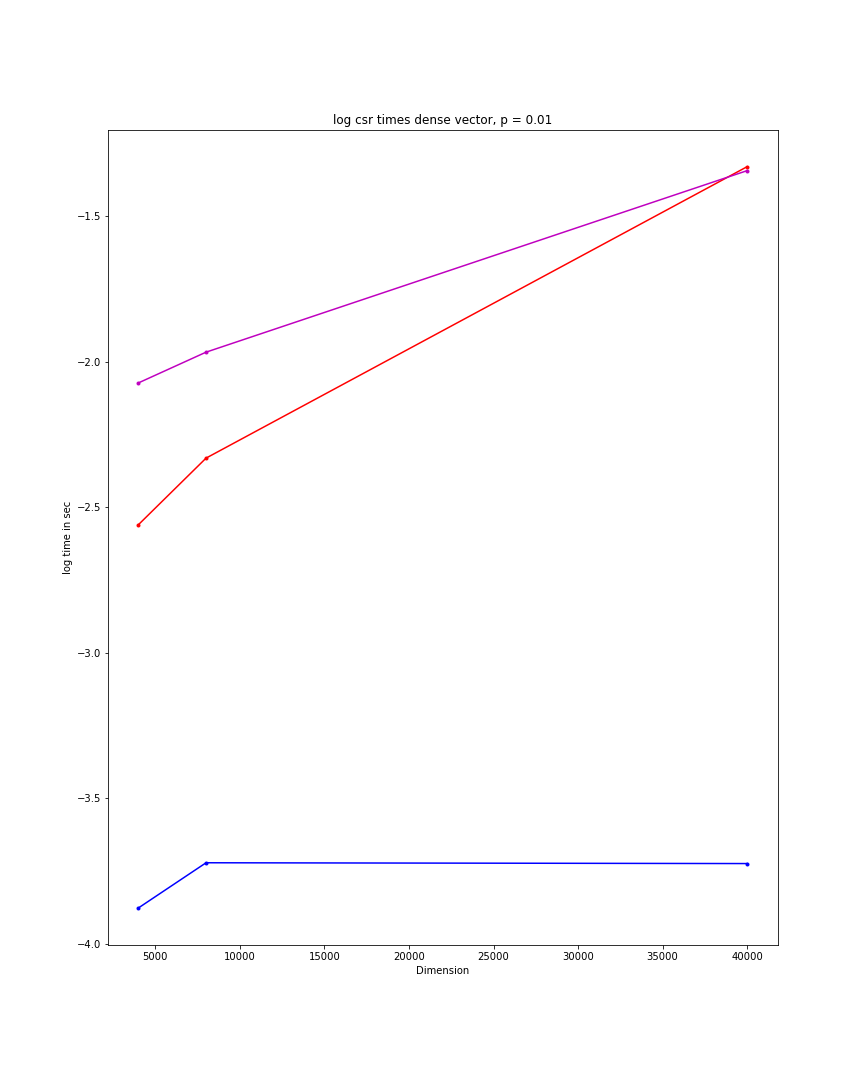
\includegraphics[scale = 0.16]{log_csr_dv_01.png}
  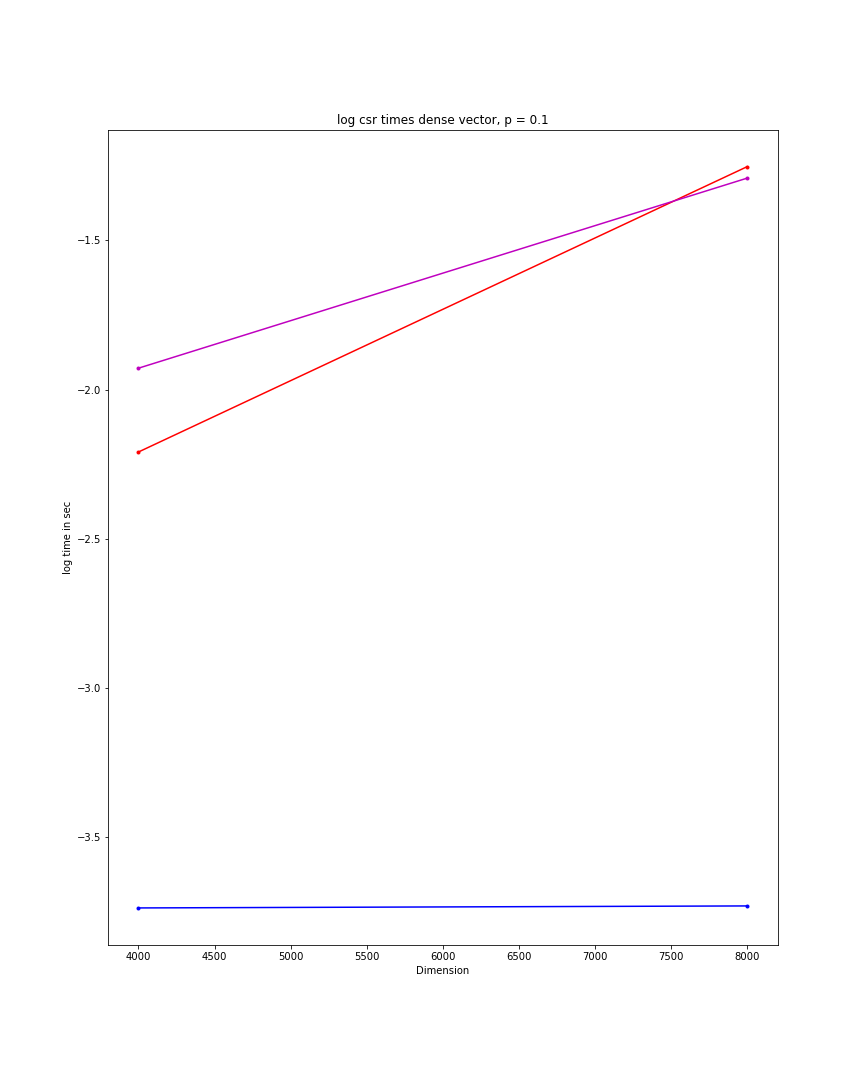
\includegraphics[scale = 0.16]{log_csr_dv_1.png}

\end{figure}

\pagebreak 




\end{document}
